\documentclass[11pt,letterpaper,oneside]{article}
%%%%%%%%%%%%%%%%%%%%%%%%%%%%%%%%%%%%%%%%%%%%%%
% GENERAL PACKAGES
%%%%%%%%%%%%%%%%%%%%%%%%%%%%%%%%%%%%%%%%%%%%%%

%\usepackage{epsfig}
\usepackage{subfigure}
\usepackage{url}
\urlstyle{sf}	% typeset urls in sans-serif

%\usepackage{amsmath}
%\usepackage{amsfonts}
%\usepackage{color}
%\usepackage{framed}

%\usepackage{makeidx}  % allows for indexgeneration
\usepackage{bm}
\usepackage{graphicx}
\usepackage[boxed, algoruled, vlined, linesnumbered]{algorithm2e} % noresetcount
\usepackage{times}
\usepackage{dsfont}
\usepackage[longnamesfirst,numbers]{natbib} %FH: longnamesfirst does not seem to work :(
\usepackage{microtype}
%\usepackage[longnamesfirst]{natbib}
\usepackage{amsmath, amssymb, amsfonts}

%Next 7 lines: tell natbib not to put bibliography onto new page
\makeatletter
\renewcommand\bibsection%
{
  \section*{\refname
    \@mkboth{\MakeUppercase{\refname}}{\MakeUppercase{\refname}}}
}
\makeatother

%% Define a new style for URLs that will use a smaller font.
%% use a different one for footnotes (requires manual switching)
\makeatletter
\def\url@newstyle{%
  \@ifundefined{selectfont}{\def\UrlFont{\sf}}{\def\UrlFont{\small}}}
\def\url@newFNstyle{%
  \@ifundefined{selectfont}{\def\UrlFont{\sf}}{\def\UrlFont{\scriptsize}}}
\makeatother
\urlstyle{new}


\newcommand{\todo}[1]{\textbf{TODO: #1}}
\newcommand{\todocrc}[1]{\note{TODOCRC: #1}}
\newcommand{\cmnt}[1]{\textbf{COMMENT: #1}}
\newcommand{\fhcrc}[1]{\note{FH CRC comment: #1}}


\newcommand{\SingleInstSaps}{{\small{\texttt{\textsc{Single\-Inst\-Saps}}}}}
\newcommand{\SingleInstSpear}{{\small{\texttt{\textsc{Single\-Inst\-Spear}}}}}
\newcommand{\Broad}{{\small{\texttt{\textsc{Broad}}}}}
\renewcommand{\AlTitleFnt}[1]{{\bf{}#1}}

%%%%%%%%%%%%%%%%%%%%%%%%%%%%%%%%%%%%%%%%%%%%%%
% CONVENIENT COMMANDS for commenting text
%%%%%%%%%%%%%%%%%%%%%%%%%%%%%%%%%%%%%%%%%%%%%%
\newcommand{\hide}[1]{}
\newcommand{\fh}[1]{{\bf{}FH: #1}}
\newcommand{\hh}[1]{\note{HH says: #1}}
\renewcommand{\hh}[1]{}
\newcommand{\klb}[1]{{\bf{}KLB: #1}}



%Configurators
\newcommand{\algofont}[1]{{\footnotesize{\textsc{#1}}}}
\newcommand{\paramils}{\algofont{Param\-ILS}}
%\newcommand{\paramils}{\textsc{Param\-ILS}}
\newcommand{\focusedils}{\algofont{Focused\-ILS}}
\newcommand{\basicils}{\algofont{Basic\-ILS}}
\newcommand{\gga}{\algofont{GGA}}
\newcommand{\smac}{\algofont{SMAC}}
\newcommand{\roar}{\algofont{ROAR}}
\newcommand{\tbspo}{\algofont{TB-SPO}}
\newcommand{\spop}{{\algofont{SPO$^+$}}}
\newcommand{\randomstar}{\algofont{Ran\-dom$^*$}}
\newcommand{\randomsearchstar}{\randomstar}
\newcommand{\frace}{{\algofont{F-Race}}}

\newcommand{\salgofont}[1]{{\scriptsize{\textsc{#1}}}}
\newcommand{\sgga}{\salgofont{GGA}}
\newcommand{\ssmac}{\salgofont{SMAC}}
\newcommand{\sroar}{\salgofont{ROAR}}
\newcommand{\stbspo}{\salgofont{TB-SPO}}
\newcommand{\sspop}{{\salgofont{SPO$^+$}}}

%SAT solvers
\newcommand{\spear}{\algofont{SPEAR}}
\newcommand{\saps}{\algofont{SAPS}}
\newcommand{\satenstein}{\algofont{SATenstein}}

%MIP solvers
\newcommand{\lpsolve}{\algofont{lp\-solve}}
\newcommand{\gurobi}{\algofont{Gu\-ro\-bi}}
\newcommand{\cplex}{\algofont{CPLEX}}
\newcommand{\ibmcplex}{\algofont{IBM ILOG CPLEX}}

%Instance sets
\newcommand{\shoe}{\textsc{SHOE}}
%\newcommand{\MASS}{\textsc{MASS}}
\newcommand{\QCP}{QCP}
\newcommand{\SWGCP}{SWGCP}
\newcommand{\MASS}{MASS}
\newcommand{\MIK}{MIK}
\newcommand{\CLS}{CLS}
\newcommand{\MJA}{MJA}
\newcommand{\corlat}{\textsc{CORLAT}}
\newcommand{\regionsonehundred}{\textsc{Regions100}}
\newcommand{\regionstwohundred}{\textsc{Regions200}}
\newcommand{\regionsseventy}{\textsc{Regions70}}

\newcommand{\SPEARSWGCP}{{\footnotesize{\texttt{\textsc{Spear-SWGCP}}}}}
\newcommand{\SPEARQCP}{{\footnotesize{\texttt{\textsc{Spear-QCP}}}}}

\newcommand{\SAPSSWGCP}{{\footnotesize{\texttt{\textsc{Saps-SWGCP}}}}}
\newcommand{\SAPSSWGCPhomog}{{\footnotesize{\texttt{\textsc{Saps-SW-hom}}}}}

\newcommand{\cplexregionsonehundred}{{\footnotesize{\texttt{\textsc{CPLEX-Regions100}}}}}
\newcommand{\cplexmik}{{\footnotesize{\texttt{\textsc{CPLEX-MIK}}}}}
\newcommand{\SAPSQCP}{{\footnotesize{\texttt{\textsc{Saps-QCP}}}}}
\newcommand{\SAPSQCPeasy}{{\footnotesize{\texttt{\textsc{Saps-QCP-easy}}}}}
\newcommand{\SAPSQCPmed}{{\footnotesize{\texttt{\textsc{Saps-QCP-med}}}}}
\newcommand{\SAPSQCPseventyfive}{{\footnotesize{\texttt{\textsc{Saps-QCP-q075}}}}}
\newcommand{\SAPSQCPninetyfive}{{\footnotesize{\texttt{\textsc{Saps-QCP-q095}}}}}
\newcommand{\SAPSSWGCPmed}{{\footnotesize{\texttt{\textsc{Saps-SWGCP-med}}}}}
\newcommand{\SAPSSWGCPseventyfive}{{\footnotesize{\texttt{\textsc{Saps-SWGCP-q075}}}}}
\newcommand{\SAPSSWGCPninetyfive}{{\footnotesize{\texttt{\textsc{Saps-SWGCP-q095}}}}}

\newcommand{\cplexregionsonehundredtiny}{\scriptsize{\texttt{\textsc{CPLEX-Regions100}}}}
\newcommand{\cplexmiktiny}{{\scriptsize{\texttt{\textsc{CPLEX-MIK}}}}}
\newcommand{\SAPSQCPtiny}{{\scriptsize{\texttt{\textsc{Saps-QCP}}}}}
\newcommand{\SPEARSWGCPtiny}{{\scriptsize{\texttt{\textsc{Spear-SWGCP}}}}}
\newcommand{\SPEARQCPtiny}{{\scriptsize{\texttt{\textsc{Spear-QCP}}}}}
\newcommand{\SAPSSWGCPtiny}{{\scriptsize{\texttt{\textsc{Saps-SWGCP}}}}}


\newcommand{\SAPSQCPmedtiny}{{\scriptsize{\texttt{\textsc{Saps-QCP-med}}}}}
\newcommand{\SAPSQCPseventyfivetiny}{{\scriptsize{\texttt{\textsc{Saps-QCP-q075}}}}}
\newcommand{\SAPSQCPninetyfivetiny}{{\scriptsize{\texttt{\textsc{Saps-QCP-q095}}}}}
\newcommand{\SAPSSWGCPmedtiny}{{\scriptsize{\texttt{\textsc{Saps-SWGCP-med}}}}}
\newcommand{\SAPSSWGCPseventyfivetiny}{{\scriptsize{\texttt{\textsc{Saps-SWGCP-q075}}}}}
\newcommand{\SAPSSWGCPninetyfivetiny}{{\scriptsize{\texttt{\textsc{Saps-SWGCP-q095}}}}}

\newcommand{\SAPSQWH}{{\footnotesize{\texttt{\textsc{Saps-QWH}}}}}
\newcommand{\SAPSQWHtiny}{{\scriptsize{\texttt{\textsc{Saps-QWH}}}}}


\newcommand{\SPEARIBMtwentyfive}{{\footnotesize{\texttt{\textsc{Spear-IBM-q025}}}}}
\newcommand{\SPEARIBMmed}{{\footnotesize{\texttt{\textsc{Spear-IBM-med}}}}}
\newcommand{\SPEARSWVmed}{{\footnotesize{\texttt{\textsc{Spear-SWV-med}}}}}
\newcommand{\SPEARSWVseventyfive}{{\footnotesize{\texttt{\textsc{Spear-SWV-q075}}}}}
\newcommand{\SPEARSWVninetyfive}{{\footnotesize{\texttt{\textsc{Spear-SWV-q095}}}}}

\newcommand{\SPEARIBMtwentyfivetiny}{{\scriptsize{\texttt{\textsc{Spear-IBM-q025}}}}}
\newcommand{\SPEARIBMmedtiny}{{\scriptsize{\texttt{\textsc{Spear-IBM-med}}}}}
\newcommand{\SPEARSWVmedtiny}{{\scriptsize{\texttt{\textsc{Spear-SWV-med}}}}}
\newcommand{\SPEARSWVseventyfivetiny}{{\scriptsize{\texttt{\textsc{Spear-SWV-q075}}}}}
\newcommand{\SPEARSWVninetyfivetiny}{{\scriptsize{\texttt{\textsc{Spear-SWV-q095}}}}}



%%%%%%%%%%%%%%%%%%%%%%%%%%%%%%%%%%%%%%%%%%%%%%
% ABBREVIATIONS
%%%%%%%%%%%%%%%%%%%%%%%%%%%%%%%%%%%%%%%%%%%%%%
\newcommand{\etal}[0]{et al.{}}
\newcommand{\eg}[0]{\emph{e.{}g.{}}}
\newcommand{\ie}[0]{\emph{i.{}e.{}}}
\newcommand{\adhoc}[0]{\emph{ad hoc}}
\newcommand{\cf}[0]{cf.{}}
\newcommand{\vs}[0]{\emph{vs}}
\newcommand{\wrt}[0]{w.{}r.{}t.{}}
\newcommand{\wrtl}[0]{with respect to}
\newcommand{\iid}[0]{i.{}i.{}d.{}}
\newcommand{\naive}[0]{na\"ive}
\newcommand{\Naive}[0]{Na\"ive}

%Math
\newcommand{\vTheta}{{\bm{\Theta}}}
\newcommand{\vtheta}{{\bm{\theta}}}
\newcommand{\vo}{{\bm{o}}}
\newcommand{\calM}{\mbox{${\cal M}$}}
\newcommand{\calD}{\mbox{${\cal D}$}}
\newcommand{\gauss}{\mbox{${\cal N}$}}
\newcommand\transpose{{\textrm{\tiny{\sf{T}}}}}

%% keep figures from going onto a page by themselves
\renewcommand{\topfraction}{0.9}
\renewcommand{\textfraction}{0.1}
\renewcommand{\floatpagefraction}{0.85}


%%%%%%%%%%%%%%%%%%%%%%%%%%%%%%%%%%%%%%%%%%%%%%
% SET UP CHANGEBAR
%%%%%%%%%%%%%%%%%%%%%%%%%%%%%%%%%%%%%%%%%%%%%%

\usepackage[outerbars,color]{changebar}
%\ifx\pdfoutput\undefined
%\else\ifnum\pdfoutput>0
%\usepackage{pdfcolmk}
%\fi\fi

\setcounter{changebargrey}{60}
\cbcolor{red}

\newcommand{\cb}[1]{\cbstart{#1} \cbend}
%\renewcommand{\cb}[1]{#1}
\newcommand{\cbgreen}[1]{\cbstart{\textcolor{green}{#1}} \cbend}
\newcommand{\tred}[1]{\textcolor{red}{#1}}


\newcommand{\denselist}{\itemsep -1.5pt\partopsep -20pt}



%%%%%%%%%%%%%%%%%%%%%%%%%%%%%%%%%%%%%%%%%%%%%%
% CONVENIENT COMMANDS for formulae
%%%%%%%%%%%%%%%%%%%%%%%%%%%%%%%%%%%%%%%%%%%%%%

\newcommand{\nangbra}[1]{$\langle{}$#1$\rangle$}
\newcommand{\angbra}[1]{\langle{}#1\rangle}
\newcommand{\bra}[1]{\left(#1\right)}
\newcommand{\squbra}[1]{\left[#1\right]}
\newcommand{\vctm}[1]{\boldmath{$#1$}\unboldmath{}}
\newcommand{\vct}[1]{\mbox{\boldmath{$#1$}\unboldmath{}}}
%\newcommand{\qed}{~\vspace*{-0.5cm}\hspace*{\textwidth}\qedsymbol~\vspace*{0.5cm}}


%%%%%%%%%%%%%%%%%%%%%%%%%%%%%%%%%%%%%%%%%%%%%%
% COMMANDS for algorithm2e.
%%%%%%%%%%%%%%%%%%%%%%%%%%%%%%%%%%%%%%%%%%%%%%
\SetCommentSty{textit}
\SetKwComment{fhcomment}{// ===== }{}
\newcommand{\nlcom}[1]{{\BlankLine\footnotesize{\fhcomment{\CommentSty{#1}}}}}
\newcommand{\com}[1]{{\footnotesize{\CommentSty{// #1}}}}

\newcommand{\fhem}[1]{\text{\emph{#1}}}
\newcommand{\algo}[2]{#1\;\small #2}

%\newcommand{\Input}[1]{Input: #1}
%\newcommand{\Output}[1]{Output: #1}
%\newcommand{\Effect}[1]{Effect: #1}

\SetKwBlock{Procedure}{begin}{end}
\SetKwFunction{Term}{TerminationCriterion()}
\SetKwFunction{Init}{GenerateInitialSolution}
\SetKwFunction{Acc}{AcceptanceCriterion}
\SetKwFunction{Best}{best}
\SetKwFunction{IteratedLocalsearch}{IteratedLocalsearch}
\SetKwFunction{Localsearch}{LocalSearch}
\SetKwFunction{IterativeFirstImprovement}{IterativeFirstImprovement}
\SetKwFunction{Pert}{Perturbation}
%\DontPrintSemicolon
\SetFuncSty{textit}

%%%%%%%%%%%%%%%%%%%%%%%%%%%%%%%%%%%%%%%%%%%%%%
% COMMANDS for theorems, lemmas, definitions, etc.
%%%%%%%%%%%%%%%%%%%%%%%%%%%%%%%%%%%%%%%%%%%%%%

%\usepackage{amsmath, amsthm, amssymb}
\newtheorem{thm}{Theorem}%[section]
\newtheorem{ex}{Example}%[section]
\newtheorem{lem}[thm]{Lemma}
\newtheorem{cor}[thm]{Corollary}
\newtheorem{obs}[thm]{Observation}

%\theoremstyle{definition}
\newtheorem{define}[thm]{Definition}
\hyphenation{ge-ne-ral-ize}

%%%%%%%%%%%%%%%%%%%%%%%%%%%%%%%%%%%%%%%%%%%%%%
% FIGURES
%%%%%%%%%%%%%%%%%%%%%%%%%%%%%%%%%%%%%%%%%%%%%%

\newcommand{\largequadraticgraph}[1]{
%        \includegraphics[width=3.9cm,height=3.9cm]{#1}
%        \includegraphics[width=4.6cm,height=4.6cm]{#1}
%        \includegraphics[width=4.9cm,height=4.6cm]{#1}
%        \includegraphics[width=5.4cm,height=5.4cm]{#1}
        \includegraphics[width=5.4cm,height=5.4cm]{#1}
  }


\newcommand{\smallquadraticgraph}[1]{
%        \includegraphics[width=3.9cm,height=3.9cm]{#1}
%        \includegraphics[width=4.6cm,height=4.6cm]{#1}
        \includegraphics[width=4.9cm,height=4.6cm]{#1}
%        \includegraphics[width=5.4cm,height=5.4cm]{#1}
}


\newcommand{\quadraticgraph}[1]{
%        \includegraphics[width=4.1cm,height=4.1cm]{#1}
        %\includegraphics[width=4.6cm,height=4.6cm]{#1}
        \includegraphics[width=5.4cm,height=5.4cm]{#1}
        %\includegraphics[width=6.15cm,height=6.15cm]{#1}
}

\newcommand{\smallgraph}[1]{
%        \includegraphics[width=6.15cm,height=4.1cm]{#1}
        %\includegraphics[width=6.9cm,height=4.6cm]{#1}
%        \includegraphics[width=12cm,height=8cm]{#1}
\includegraphics[width=5.4cm,height=3.6cm]{#1}
%	\includegraphics[width=4.95cm,height=3.3cm]{#1}
}


\newcommand{\normalgraph}[1]{
%        \includegraphics[width=6.15cm,height=4.1cm]{#1}
        \includegraphics[width=6.9cm,height=4.6cm]{#1}
%        \includegraphics[width=12cm,height=8cm]{#1}
%\includegraphics[width=5.4cm,height=3.6cm]{#1}
%	\includegraphics[width=4.95cm,height=3.3cm]{#1}
}

\newcommand{\biggergraph}[1]{
%        \includegraphics[width=6.15cm,height=4.1cm]{#1}
        \includegraphics[width=6.9cm,height=4.6cm]{#1}
%        \includegraphics[width=12cm,height=8cm]{#1}
%\includegraphics[width=5.4cm,height=3.6cm]{#1}
%	\includegraphics[width=4.95cm,height=3.3cm]{#1}
}

\newcommand{\fig}[3]{  % input_file, label, caption
  \begin{figure}[tpb]
    \begin{center}
      \normalgraph{#1}
      \caption{\label{#2}#3}
    \end{center}
  \end{figure}
}


\newcommand{\qfig}[3]{  % input_file, label, caption
  \begin{figure}[tpb]
%hh: temporarily changed:
%  \begin{figure}[p]
    \begin{center}
      \quadraticgraph{#1}
      \caption{\label{#2}#3}
    \end{center}
  \end{figure}
}

\newcommand{\largeqfig}[3]{  % input_file, label, caption
%  \begin{figure}[tpb]
%hh: temporarily changed:
  \begin{figure}[p]
    \begin{center}
      \largequadraticgraph{#1}
      \caption{\label{#2}#3}
    \end{center}
  \end{figure}
}

\newcommand{\sides}[6]{         %fig1, fig2, cap1, cap2, cap, label
        \begin{figure*}[tbph]
        \hfill
            \subfigure[#3]
            {
                \quadraticgraph{#1}
                  }
        \hfill{}
        \hfill
            \subfigure[#4]
            {
                \quadraticgraph{#2}
                  }
        \hfill{}
        \caption{#5}
        \label{#6}
%        \vspace{-0.245cm}
        \end{figure*}
}

\newcommand{\threefig}[8]{         %fig1, fig2, fig3, cap1, cap2, cap3, cap, label
    \begin{figure*}[tbp]
      \begin{center}
        \mbox{
            \subfigure[#4]
            {
                \quadraticgraph{#1}
                  }
            \subfigure[#5]
            {
                \quadraticgraph{#2}
                  }
            \subfigure[#6]
            {
                \quadraticgraph{#3}
                  }
        }
        \vspace{-0.4cm}
        \caption{#7}
        \label{#8}
      \end{center}
      \vspace{-0.245cm}
    \end{figure*}
}

\newcommand{\threebfig}[8]{         %fig1, fig2, fig3, cap1, cap2, cap3, cap, label
    \begin{figure*}[tb]
      \begin{center}
        \mbox{
            \subfigure[#4]
            {
                \smallgraph{#1}
                  }
            \subfigure[#5]
            {
                \smallgraph{#2}
                  }
            \subfigure[#6]
            {
                \smallgraph{#3}
                  }
        }
        \vspace{-0.4cm}
        \caption{#7}
        \label{#8}
      \end{center}
      \vspace{-0.245cm}
    \end{figure*}
}

\usepackage{fullpage}
\usepackage{setspace}
\usepackage{subfiles}
\usepackage{graphicx}
%%\usepackage{hyperref}
\usepackage{listings}
\usepackage{tablefootnote}
\usepackage{amssymb}
\usepackage{textcomp}
\usepackage{mathrsfs}
\usepackage{color}
\usepackage{longtable}
\usepackage{hyperref}

\usepackage{lipsum}
\usepackage[svgnames]{xcolor}
\usepackage[tikz]{bclogo}


\newcommand{\note}[1]{}
% comment the next line to turn off notes
\renewcommand{\note}[1]{~\\\frame{\begin{minipage}[c]{\textwidth}\vspace{2pt}\center{#1}\vspace{2pt}\end{minipage}}\vspace{3pt}\\}


\begin{document}

\title{Manual for MySQL Target Algorithm Evaluator }
\author{
Steve~Ramage\\
Department of Computer Science\\
University of British Columbia\\
Vancouver, BC\ \ V6T~1Z4, Canada\\
\texttt{\{seramage\}@cs.ubc.ca}
}


\maketitle

\tableofcontents

%%%%%%%%%%%%%%%%%%%%%%%%%%%%%%%%%%%%%%%%%%%%%%%%%%%%%%%%%%%%%%%%%%%%
\section{Introduction}
%%%%%%%%%%%%%%%%%%%%%%%%%%%%%%%%%%%%%%%%%%%%%%%%%%%%%%%%%%%%%%%%%%%%

The MySQL Target Algorithm Evaluator is an implementation of AEATK's \texttt{TargetAlgorithmEvaluator} interface, that supports distributed execution through the use of a centralized MySQL Database. This document is designed to read by two types of users:

\begin{enumerate}
\item Users who would like to use the workers as part of an existing AEATK application
\item Developers of AEATK applications who would like to make them compatible with the workers.
\end{enumerate}

\subsection{License}

The MySQL Target Algorithm Evaluator has been released under the AGPLv3 license. Please contact Frank Hutter \texttt{hutter@cs.ubc.ca} to discuss other licensing opportunities.

%%%%%%%%%%%%%%%%%%%%%%%%%%%%%%%%%%%%%%%%%%%%%%%%%%%%%%%%%%%%%%%%%%%%
\section{Usage}
%%%%%%%%%%%%%%%%%%%%%%%%%%%%%%%%%%%%%%%%%%%%%%%%%%%%%%%%%%%%%%%%%%%%

%%%%%%%%%%%%%%%%%%%%%%%%%%%%%%%%%%%%%%%%%%%%%%%%%%%%%%%%%%%%%%%%%%%%
\subsection{Prerequisites}
%%%%%%%%%%%%%%%%%%%%%%%%%%%%%%%%%%%%%%%%%%%%%%%%%%%%%%%%%%%%%%%%%%%%

\subsubsection{User Prerequisites}

To use the MySQL Target Algorithm Evaluator it is expected that you are familiar with the following concepts:

\begin{enumerate}

\item You are familiar with the basics of the AEATK \emph{wrapper} interface. Specifically you are aware that an algorithm will be invoked via the command line given an instance, cutoff time, seed and a parameter configuration, and the wrapper of the algorithm will return a status flag as well as measurements of runtime, runlength, quality, and some additional run data. This is key, since this project essentially allows for distributing the execution of these wrappers.

\item You know how to connect to a MySQL Server using the \texttt{mysql} command.

\item You can execute basic \texttt{SELECT} and \texttt{UPDATE} statements as necessary. A good tutorial on SQL is available here: \url{http://www.w3schools.com/sql/sql\_syntax.asp}

\item You can create a database in MySQL.

\item It is expected that you read through this entire document (end-to-end). In 90\%-95\% of cases, the MySQL Target Algorithm Evaluator can be used without a second thought but you should be familiar with this document, as occasionally you will need to understand the architectural limitations.

\end{enumerate}

\subsubsection{System Prerequisites}

It is assumed that you have access to a MySQL Server running version 5.5. Version 5.1 may or may not work. MariaDB and MySQL 5.6 should work but have never been tested. Additionally you must have access to a user and database that allows for \texttt{SELECT, INSERT, UPDATE, DELETE} as well as \texttt{CREATE TABLE} permissions.

%\begin{bclogo}[logo=\bcattention, noborder=false, barre=none]{Important!}
%    \lipsum[1]
%\end{bclogo}
\begin{bclogo}[logo=\bcattention, couleurBarre=red, noborder=true]{Important!}
Good performance of the MySQL Target Algorithm Evaluator depends \emph{heavily} on the MySQL Server being tuned correctly. Unfortunately the default configuration of MySQL Server is incredibly inappropriate. More advanced users are encouraged to read Chapter 8 of \emph{High Performance MySQL 3rd Edition}.  Assuming that you are only interested in using MySQL for this application and are not running anything else, we would recommend the following changes (if you are using MySQL for something else, you will need to do your own research).

The three most important settings to change are:

\begin{itemize}
\item \texttt{innodb\_buffer\_pool\_size} which should be set to 80\% of the RAM you would like MySQL to use (we use 16 GB). For more information see: \\ \url{http://dev.mysql.com/doc/refman/5.5/en/innodb-parameters.html\#sysvar\_innodb\_buffer\_pool\_size}

\item \texttt{innodb\_log\_file\_size} which should be set to about 1 GB or higher.  For more information see: \\
\url{http://dev.mysql.com/doc/refman/5.5/en/innodb-parameters.html\#sysvar\_innodb\_log\_file\_size}

\item \texttt{max\_allowed\_packet} which should be set to 16 MB or higher (we set it to 64 MB). For more information see: \\
\url{http://dev.mysql.com/doc/refman/5.5/en/server-system-variables.html\#sysvar\_max\_allowed\_packet}

\end{itemize}

Additionally Section \ref{appendix:sampleconf} starting on page \pageref{appendix:sampleconf} has a sample configuration that we use.

\end{bclogo}

\subsection{Overview}


\begin{figure}
\centering
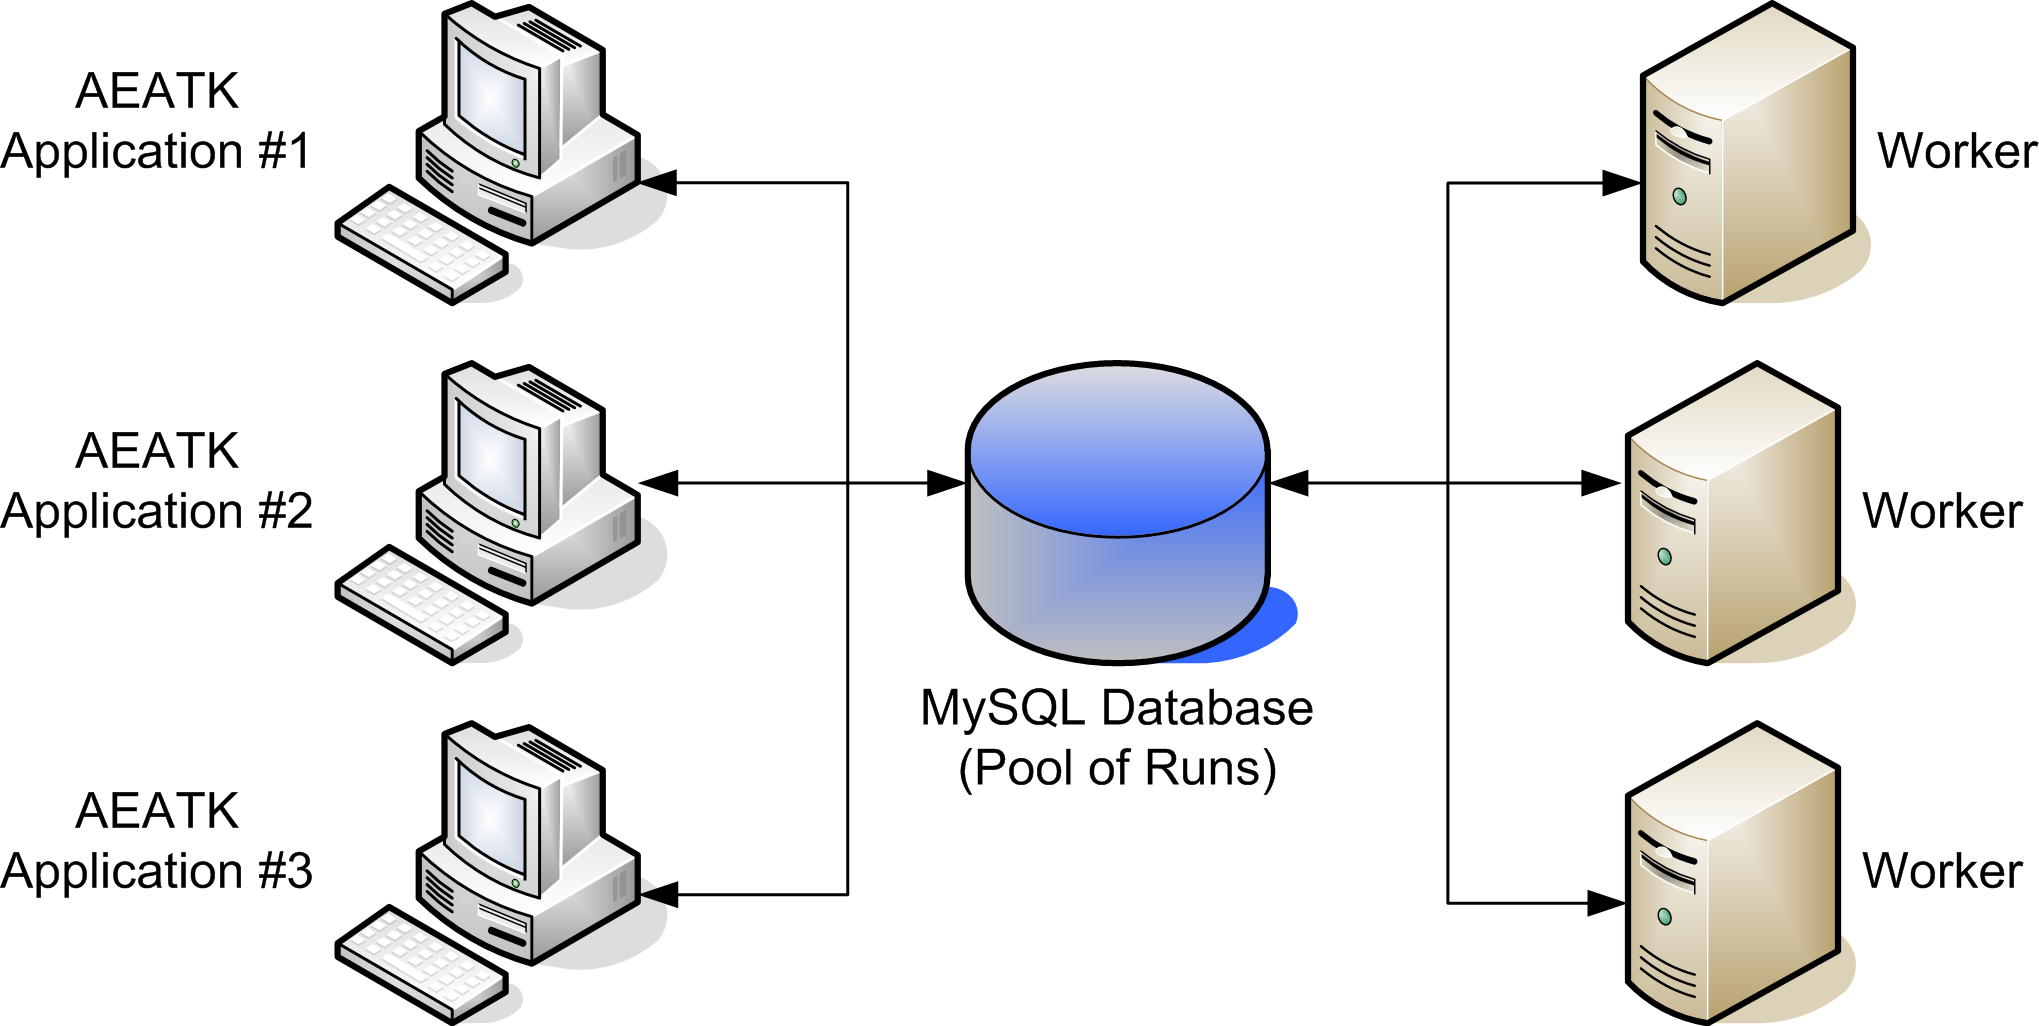
\includegraphics[scale=0.90]{img/Architecture/ArchitectureOverview}
\caption{Architecture of the MySQL Target Algorithm Evaluator}\label{arch}
\end{figure}

Both users and developers should be aware of the basic architecture, which is pictured in Figure \ref{arch}. In essence, all communication between the application and the worker is done through the database. In fact it is almost entirely \emph{anonymous}. The database structure is designed to be simple and in fact is nothing more than a glorified list of runs to execute. The application is entirely unaware about which worker, if any, executed it's run, and the worker is unaware about which application requested the run or why.  This anonymity has certain benefits like allowing for simple caching, as well as allowing users to manually intervene in the database.

\subsubsection{Database Overview} 

Beyond a simple database (in the \texttt{CREATE DATABASE} meaning of the term), the MySQL Target Algorithm Evaluator also has a concept of pools. A pool is essentially a family of tables that serve as a light weight database. For instance you might create a pool for each job id on the cluster to manage experiments, or whatever else you'd like. Workers are assigned to a pool and will operate on all runs in the pool. When executing, all table names will be prefixed with the pool name, so for instance the \texttt{runs} table with pool \texttt{test} will actually be called \texttt{test\_runs}.

For an exact detailed listing of the tables and columns consult the database. The meaning of individual columns are heavily  based on AEATK concepts and largely just a one-to-one mapping to a field in AEATK.  The following however is an overview of what is important.

\begin{bclogo}[logo=\bclampe, couleurBarre=red, noborder=true]{Suggestion}
Using PHPMyAdmin (\url{www.phpmyadmin.net}) for interacting with the database can make many things much easier. Ask your system administrator to install it for you.

\end{bclogo}

\begin{description}

\item[commandTable]	 This table simple lists all AEATK applications commands that were executed if available. Data is never read from this table, and mainly exists in case the command that generated the data has been forgotten.

\item[version] This table simply lists the version of the MySQL Target Algorithm Evaluator that created the table. The hash is actually a hash of the file that creates the tables. If the hash that exists in the database differs from the current one a warning will be logged. This might indicate that the structure has changed and is incompatible.

\item[algoExecConfig] This table contains information about executing the algorithm, it's location, it's configuration space, etc. It is inserted into once. All of the fields are informational and are just used to recreate the appropriate AEATK object in the worker. For AEATK users, it is the \texttt{AlgorithmExecutionConfiguration} object and the \texttt{ParameterConfigurationSpace} object that is stored here.

\item[runs] This table is where most of the magic happens\footnote{For database aficionados, this table is roughly a denormalized version of three sets of information, the information necessary to execute the run, the result of the run, and information controlling the run status. It has been denormalized for both performance and ease of use for users. This table is hit very heavily}. The remaining information necessary to reconstruct an call to the wrapper is here.  Other columns of note are:

\begin{center}
\begin{tabular}{p{3.5cm} | p{11.5cm} }
Column & Description \\
\hline
\hline
runHashCode & The hash is a SHA1 hash of key information that identifies the run. The hash is only used by the AEATK Application portion. It is \emph{approximately} (You should consult the code for the authoritative calculation) the instance name, seed, cutoff, parameter configuration, and the execConfig all concatenated as a string and then and hashed. Some other options also affect the hash, such as the runPartition (described below).\\
\hline 
status & Controls the current status of a run (either \texttt{NEW}, \texttt{ASSIGNED}, or \texttt{COMPLETE}). \\
\hline
priority & Allows for rudimentary control of the priority of the run. In the AEATK application you can set the \textbf{-$~\!$-mysqldbtae-priority} option to control this, or manually alter it in the table. Higher priorities are selected first for processing.\\
\hline
killJob & Flag that signifies whether the application requested the run be terminated. \\
\hline 
retryAttempts & Stores the number of times a worker was assigned the run since the last time it was requested. \\
\hline 
runPartition & A unique integer that allows for different AEATK applications to interact with the same pool \emph{without} using the same cache. Each one can be assigned a different \textbf{-$~\!$-mysqldbtae-run-partition} which will cause different hashes to be generated.  \\
\hline
worstCaseEndtime & An approximate, pessimistic and informational-only estimate of the latest time a run could complete. \\
\hline
worstCaseNextUpdate\_ WhenAssigned & If the run is \texttt{ASSIGNED} and this time is in the past, then we expect that the run will not be completed, and may be reclaimed. \\
\hline
\end{tabular}
\end{center}

\begin{bclogo}[logo=\bcattention, couleurBarre=red, noborder=true]{Important!}
Executing queries against this table while the workers are running needs to be done with care as you may inadvertently stall the workers, especially when this table contains millions of records. 
\end{bclogo}


\item[workers]

This table controls the status of the workers, and allows for online management of the workers. Many of the fields are  strictly informational including the \texttt{hostname}, \texttt{jobID}, \texttt{status}, \texttt{version}, \texttt{startTime}, \texttt{startWeekYear}, \texttt{orginalEndTime}. Additionally other fields contain the suffix \texttt{\_UPDATEABLE} this means that if you change this value \textsc{AND} change the value of \texttt{upToDate} to 0, the worker will re-read this value and change it's behaviour.


Many of these columns values can be initially set on the command line of the worker via the appropriate argument.

Some columns of note are (Note we have removed the \texttt{\_UPDATEABLE} suffix here for space reasons):

\begin{center}
\begin{tabular}{p{3.5cm} | p{11.5cm} }
Column & Description \\
\hline
\hline
autoAdjustBatchSize & If true then the worker will slowly increase the number of runs it requests (the \texttt{runsToBatch} column) from the database in batches if it is idle, if it can't get as many runs as it requests it will request fewer runs.  The minimum and maximum size are controlled by the other columns.  \\
\hline 
delayBetweenRequests & This is loosely how often the workers will poll for new runs, if all runs the worker was assigned finished before this, it will wait until this amount of time expires before continuing. \\
\hline
poolIdleTimeLimit & If the sum of all the \texttt{workerIdleTime} values within the past few \texttt{startWeekYears} exceeds this value, and this worker becomes idle, it will terminate to avoid wasting cluster time.\\
\hline
concurrencyFactor & This is the number of workers that can simultaneously hold a lock on the \texttt{runs} table. Setting this too high can result in performance problems.\\
\hline
pool & If changed the workers will restart on another pool, if that pool doesn't exist the worker MAY die depending on other options. \\
\hline
worstCaseNextUpdate\_ WhenRunning & If this value is ever in the past and the worker has status \texttt{RUNNING}, then we assume the worker has died. \\
\hline 

\end{tabular}
\end{center}

\end{description}

\subsubsection{AEATK Application}

\begin{figure}
\centering
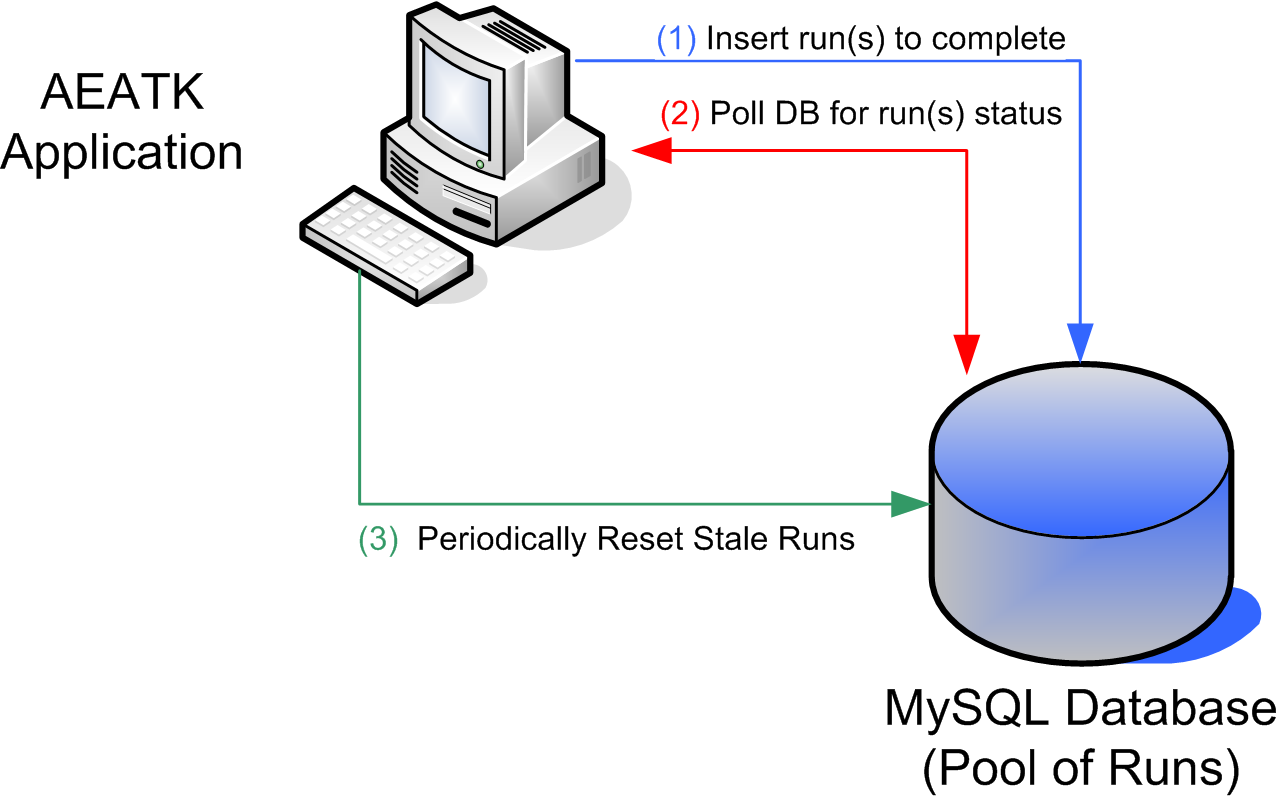
\includegraphics[scale=1]{img/Architecture/Master}
\caption{Master - Database Interactions}\label{master}
\end{figure}

Because neither the workers nor the application are aware of each other, it helps to think about their responsibilities / processes separately. Figure \ref{master} contains a diagram of the responsibilities and interactions of the application and the database.

\begin{enumerate}
\item The runs are inserted into the database. The MySQL Target Algorithm Evaluator uses hashing to reuse runs. If a run already exists it is reused as is. At a certain points a run may be interrupted or killed, if the run was killed or the wrapper signalled an \textbf{ABORT}, the cached run will \textsc{not} be used, and instead it will be run again.

\item Periodically the database is queried to see if the runs were completed (i.e., \textbf{status} is \texttt{COMPLETED}, if so they are returned.

\item Periodically the application checks the \texttt{runs} and \texttt{workers} tables for columns that have not been updated by the correct time (given by the corresponding \texttt{worstCaseNextUpdate} time). Entries in the \texttt{workers} table will have their status set to \texttt{DONE}, where as entries in the \texttt{runs} table will be set to \texttt{NEW} status.

\end{enumerate}



\subsubsection{Worker}

\begin{figure}
\centering
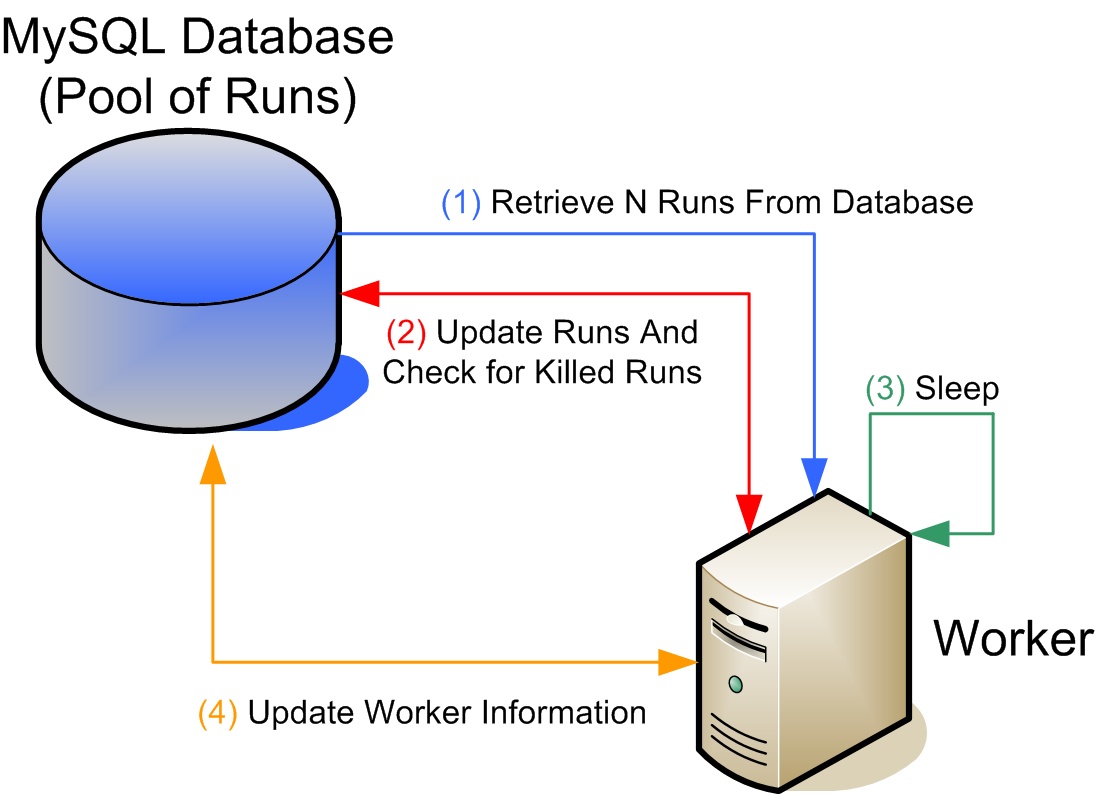
\includegraphics[scale=1]{img/Architecture/Worker}
\caption{Worker - Database Interactions}\label{worker}
\end{figure}

Figure \ref{worker} outlines the interactions between the workers and the database. 

\begin{enumerate}
\item The worker retrieves $N$ runs from the database which can be controlled via the \textbf{-$~\!$-runs-to-batch} and related options on the worker command line.
\item The worker processes each runs one at a time, periodically updating the database and checking if the run should be killed. For AEATK developers, this happens when the worker's \texttt{TargetAlgorithmEvaluator} triggers the observer. If observation isn't supported by the \texttt{TargetAlgorithmEvaluator} then this will not occur.
\item The worker then sleeps out the remaining time on delays between requests. 
\item The worker periodically checks the workers table to see if its row has and \texttt{upToDate} set to 0, if so it refreshes the parameters, and takes any action as appropriate. After this step, if any runtime limits have been reached the worker will exit.
\end{enumerate}

%%%%%%%%%%%%%%%%%%%%%%%%%%%%%%%%%%%%%%%%%%%%%%%%%%%%%%%%%%%%%%%%%%%%
\subsection{Basic}
%%%%%%%%%%%%%%%%%%%%%%%%%%%%%%%%%%%%%%%%%%%%%%%%%%%%%%%%%%%%%%%%%%%%

This section will outline the basic usage of the MySQL Target Algorithm Evaluator with a sample AEATK application, that is included with the MySQL Target Algorithm Evaluator package. The application performs random evaluations of the branin function (see \url{http://www.sfu.ca/~ssurjano/branin.html}) and reports the minimum value found out of all evaluated. Other AEATK applications should have the same command line interface, and so by following the same steps here in the other application you should be able to run that application in a distributed setting.

As stated previously it is assumed that you are familiar with the wrapper execution, if not please consult Section 5 of the SMAC Manual. The wrapper included is based on the wrapper included within SMAC, and requires python to be installed. The branin function has a global function minimum of $0.397887$ which occurs at $(-\pi, 12.275), (\pi, 2.275)$ and $(9.42478, 2.475)$.

\vspace{5pt}
\textsc{Note}: This wrapper has been modified to sleep for 0.5 seconds to provide us with a more interesting example.

\vspace{5pt}
\textsc{Location}: The files for this example are in the \texttt{example} subfolder.

We can verify this by executing the wrapper directly:
\begin{verbatim}
$./branin-sleep.py null 1 0 -1 -x1 -3.141 -x2 12.275
Result of this algorithm run: SUCCESS, 0, 0, 0.397891, 0
\end{verbatim}

You can run the included program \texttt{branin-search} which will by default perform the search locally. 

\subsubsection{Running the Program Locally}


\begin{verbatim}
./branin-search
[INFO ] Starting Random Search for minimum of Branin Function
[INFO ] Branin Search has completed 1 runs out of 100
[INFO ] Branin Search has completed 26 runs out of 100
[INFO ] Branin Search has completed 51 runs out of 100
[INFO ] Branin Search has completed 76 runs out of 100
[INFO ] Best value for the Brainin Function found was: 0.593666 and occurred at 
-x1 '-3.142700170192641' -x2 '12.720123424738636'. Search took 55.796 seconds
\end{verbatim}

If you run \texttt{branin-search} you should see the output given above and it should take approximately 1 minute to execute. This program is running the algorithm via the command line, and with the above arguments is being done sequentially.

\subsubsection{Starting the workers}
\label{start-workers}

\label{running-mysqldbtae}
The first step is to create the database that will be used:
\begin{verbatim}
$mysql -h <hostname> -u <username>
mysql>CREATE DATABASE braninSearch;
Query OK, 1 row affected (0.03 sec)
\end{verbatim}

Before running our application with the MySQL Target Algorithm Evaluator we should start some workers to be able to process them. We can start them with the following command \footnote{The default port for MySQL is 3306}:

\begin{verbatim}
$mysql-worker --pool example --mysql-username <username> --mysql-password
 <password> --mysql-hostname <hostname> --mysql-port <port> --mysql-database
braninSearch --delay-between-requests 1
\end{verbatim}

\begin{bclogo}[logo=\bclampe, couleurBarre=red, noborder=true]{Suggestion}
The final argument \textbf{-$~\!$-delay-between-requests} is optional, it changes how often the database is polled. In general the default value is conservative but good enough. We are changing it here because it is too conservative for the scale and duration of this tutorial. In general it is recommended that you leave this value alone, especially at first. For more information see FAQ \ref{faq:performance}.
\end{bclogo}

The example target algorithm, \texttt{branin-sleep}, is executing a \texttt{sleep()} call and not actually using CPU processing time. As a result we can easily process these jobs even on a single core machine. I would recommend starting 8 workers to process these runs.

\subsubsection{Running with the MySQL Target Algorithm Evaluator}
We can change the \texttt{TargetAlgorithmEvaluator} implementation on the command line using the \textbf{-$~\!$-tae} argument, and supply the necessary arguments to the Target Algorithm Evaluator. This and other Target Algorithm Evaluator options are the same across this application, SMAC, and other applications. For more information see FAQ \ref{faq:verify}.

\begin{verbatim}
$./branin-search --tae MYSQLDB --mysqldbtae-pool example --mysqldbtae-username
 <username>  --mysqldbtae-password <password> --mysqldbtae-hostname <hostname>
--mysqldbtae-port <port> --mysqldbtae-database braninSearch 
\end{verbatim}

\begin{bclogo}[logo=\bclampe, couleurBarre=red, noborder=true]{Important}
Note that the worker and AEATK application use different arguments for specifying the same thing. This is because the worker is itslef an AEATK application, and consequently could use the MySQL Target Algorithm Evaluator. By default the workers will use the command line Target Algorithm Evaluator, but they can use any one, even a plugin.
\end{bclogo}

\begin{bclogo}[logo=\bclampe, couleurBarre=red, noborder=true]{Suggestion}
You can remove the need to specify the arguments for MySQL on the command line everytime using option files, see FAQ \ref{faq:optionFiles} for more information.
\end{bclogo}

After this starts executing you can verify that the runs were inserted into the database:
\begin{verbatim}
mysql> SELECT status,COUNT(*) FROM example_runs GROUP BY status; 
+----------+----------+
| status   | COUNT(*) |
+----------+----------+
| NEW      |       64 |
| ASSIGNED |       14 |
| COMPLETE |       22 |
+----------+----------+
3 rows in set (0.00 sec)
\end{verbatim}

The above indicates we are roughly 20\% completed the runs, eventually when all runs are completed the \texttt{branin-search} application should exit, and you should see the full output that is similar to the following:

\begin{verbatim}
$./branin-search --tae MYSQLDB --mysqldbtae-pool example --mysqldbtae-username 
<username> --mysqldbtae-password <password> --mysqldbtae-hostname <hostname>
 --mysqldbtae-port <port> --mysqldbtae-database braninSearch
 
[INFO ] Starting Random Search for minimum of Branin Function
[INFO ] Branin Search has completed 14 runs out of 100
[INFO ] Branin Search has completed 44 runs out of 100
[INFO ] Branin Search has completed 71 runs out of 100
[INFO ] Branin Search has completed 99 runs out of 100
[INFO ] Best value for the Brainin Function found was:
0.593666 and occurred at -x1 '-3.142700170192641' -x2 '12.720123424738636'.
Search took 10.294 seconds
\end{verbatim}

So in this case we got a 5.4$\times$ speed up. In general for very short runs the over head of the database can be pretty extreme, but is largely independent of the number of runs. For more information on how performance changes see FAQ \ref{faq:plots}.

\textsc{Note}: If we run the command again it completes almost instanteously:

\begin{verbatim}
[INFO ] Best value for the Brainin Function found was: 0.593666 and occurred at -x1 '-3.142700170192641' -x2 '12.720123424738636'. Search took 0.244 seconds
\end{verbatim}

This is a result of the caching, as all runs are complete. You can delete the runs in the database to try the search again, or you can change the \textbf{-$~\!$-seed} argument to the \texttt{branin-search} program.





%If you run the command again, you'll notice that it is much faster the second time. This is because of the caching that is done. When using the MySQL Target Algorithm Evaluator you may notice that some applications, notably the validation utility included in SMAC, actually exit before the runs are completed. You can then later rerun the utility when the runs are done, to have it generate the results. Importantly, in these applications, randomization is carefully controlled to ensure that the same sequence of runs are generated. In \texttt{branin-search} the \textbf{-$~\!$-seed} argument controls the exact configurations that are generated, and turns a randomized search algorithm into a deterministic sequence of runs.

\subsection{Installation}

Up until this point we have skipped talking about how to install the MySQL Target Algorithm Evaluator, in the above example however we didn't need to install it because it came with the MySQL Target Algorithm Evaluator.  Lets look at another example, the \texttt{algo-test} utility included in SMAC (available at \url{http://aclib.net/smac/}. Within SMAC are a number of sample scenarios, any one of them well do fine. The algo-test utility essentially does a sample algorithm run, and is useful for verifying that SMAC can run the algorithm. It is an AEATK application, and so we can change the TAE on the command line.  First lets verify that we can run it locally:

\begin{verbatim}
./util/algo-test --scenario-file ./example_scenarios/branin/branin-scenario.txt 
Starting algo-test with 128 MB of RAM
...
[INFO ] Run 0 on Instance(1):no_instance has status =>  RUNNING, 0.0
[INFO ] Run Completed
[INFO ] Run 0 on Instance(1):no_instance with config: -x1 '2.5' -x2 '7.5' _
 had the result => SAT, 0.0, 0.0, 24.129964, 1, 
\end{verbatim}

Now if we check the version of the \texttt{algo-test} utility we will see the following:
\begin{verbatim}
$./util/algo-test -v
Starting algo-test with 128 MB of RAM
**** Version Information ****
Algorithm Execution & Abstraction Toolkit ==> v2.08.01-master-776 (296fd9ab6768)
Java Runtime Environment ==> Java HotSpot(TM) 64-Bit Server VM (1.7.0_40)
OS ==> Linux 3.13.0-39-generic (amd64)
Random Forest Library ==> v1.05.01-master-108 (7fba58fe4271)
SMAC ==> v2.08.01-master-740 (217d25a4724f)
\end{verbatim}

Now copy the \emph{contents} of the \texttt{mysqldbtae-plugin} folder into the lib folder and run the same command again (still executing locally), and observe that you now see a row for the MySQL Database Target Algorithm Evaluator:

\begin{verbatim}
$./util/algo-test -v
Starting algo-test with 128 MB of RAM
**** Version Information ****
Algorithm Execution & Abstraction Toolkit ==> v2.08.01-master-776 (296fd9ab6768)
Java Runtime Environment ==> Java HotSpot(TM) 64-Bit Server VM (1.7.0_40)
MySQL Database Target Algorithm Evaluator ==> 
v0.92.00b-development-128 (b6d8a7fa90aa)
OS ==> Linux 3.13.0-39-generic (amd64)
Random Forest Library ==> v1.05.01-master-108 (7fba58fe4271)
SMAC ==> v2.08.01-master-740 (217d25a4724f)
\end{verbatim}

Now following the exact same procedure as before we can use the MySQL Target Algorithm Evaluator. First we start a worker:

\begin{verbatim}
$./lib/mysql-worker --pool example2 --mysql-username <username> --mysql-password <password> --mysql-hostname <hostname> --mysql-port <port> --mysql-database <database>
\end{verbatim}

Then we execute the utility the same as before with appropriate arguments:

\begin{verbatim}
$./util/algo-test --scenario-file ./example_scenarios/branin/branin-scenario.txt 
--tae MYSQLDB --mysqldbtae-pool example2 --mysqldbtae-username 
<username> --mysqldbtae-password <password> --mysqldbtae-hostname <hostname>
 --mysqldbtae-port <port> --mysqldbtae-database <database>
Starting algo-test with 128 MB of RAM
...
[INFO ] Run 0 on Instance(1):no_instance has status =>  SAT, 0.0
[INFO ] Run Completed
[INFO ] Run 0 on Instance(1):no_instance with config: -x1 '2.5' -x2 '7.5'
 had the result => SAT, 0.0, 0.0, 24.129964, 1,
\end{verbatim}

We can confirm that this executed in the database by running the same query:

\begin{verbatim}
mysql> SELECT status,COUNT(*) FROM example2_runs GROUP BY status; 
+----------+----------+
| status   | COUNT(*) |
+----------+----------+
| COMPLETE |        1 |
+----------+----------+
1 row in set (0.00 sec)
\end{verbatim}


\subsection{DZQ}

Included with the MySQL Target Algorithm Evaluator is the \texttt{dzq} utility, it is a utility that wraps arbitrary command line calls within the AEATK framework and executes them using workers.  At first glance this may seem quite circular and unnecessary, but in some cases this provides an advantage:

\begin{itemize}

\item If your cluster only lets you schedule some fixed number of jobs, this can allow you to avoid having to statically partition the jobs into smaller jobs.
\item If your jobs may have very small runtimes, this can lower the dispatch overhead (which in our case can be several minutes per job).
\item If your jobs may randomly fail non-deterministically, and if the scripts supply proper exit codes (0 for success, $>0$ for failure), you can monitor those jobs in the database as easily manage the failures, etc...
\item You don't have a queueing system of your own but would like one that is somewhat familiar \footnote{The author is not recommending that this be used as a queueing system, it is not, but if you were using the MySQL workers anyway}.
\end{itemize}

For more information run \texttt{dzq --help} on the command line, note that it essentially contains a built in wrapper decoder that maps the standard wrapper format to something that will call arbitrary commands. By default it uses the \texttt{CLI} Target Algorithm Evaluator, you will need to use the \texttt{MYSQLDB} one to get full benefits.

\subsection{Repair}

Included with the MySQL Target Algorithm Evaluator is the \texttt{mysql-repair} utility. This utility will upgrade some older versions of the database to the new format, and repair the hash codes of entries. The command line is pretty straight forward, again consult \textbf{-$~\!$-help} for more information. Additionally a section of the FAQ has 

\section{FAQ}

\subsection{Troubleshooting}

\subsubsection{How can I verify that the MySQL Target Algorithm Evaluator is available?}
\label{faq:verify}

This can depend on how well the applications honors certain AEATK conventions \footnote{These conventions are evolving, and undocumented, so don't blame the author of your particular application }. The first step would be to run the application with the \textbf{-v} argument and see if MySQL is listed. You can also look at the \textbf{-$~\!$-help} argument and look at the allowed values for the \textbf{-$~\!$-tae} argument, and also whether any arguments start with \textbf{-$~\!$mysqldbtae-} . If none of these are accessible then it is entirely up to the author of the application, and some applications may not expose this on the command line.

\subsection{I have really big instances, configurations, etc, and they don't seem to work.}
\label{big}

There are a couple of limits that you could run into when you have extremely large instances or configuration spaces. They generally fall into three camps, changing the column size limits, changing the batch insert size, and changing MySQLs configuration. The advice that follows presumes that this is occurring either during insertion of a runs in the AEATK application, or logging the result of a run on the worker.

There are generally two things that need to change in order for you to get this to work, the first is that you may or may not be hitting a limit on the column of a table. For instance if your problem instance is larger than 8172 characters \footnote{This was the limit at time of writing}, you may get an error when inserting it.You generally can safely increase the the limits of the table without directly causing a problem with the workers. However if you do any subsequent queries involving the column that performance may then tank (for instance if you were to change problemInstance to a TEXT, and then want to get an average runtime grouped by problemInstance, MySQL may perform horribly or may actually not let you \footnote{The author was too lazy to check which it is.}. Additionally the author believes that an InnoDB row can be at most 64 KB (or some value like this), excluding \texttt{TEXT} and \texttt{BLOB} columns. 

The next limit you may hit involves the MySQL setting \texttt{max\_allowed\_packet}. A single packet cannot exceed this value in bytes. When inserting multiple runs the MySQL Target Algorithm Evaluator will batch the insertions in sizes controlled by \textbf{-$~\!$-mysqldbtae-batch-insert-size}, at the time of writing the value of this defaulted to a conservative 500 (rows typically involve no more than 1 KB), you could lower this value almost to 1, although you pay the overhead of increased latency for database traffic.  If even 1 row cannot be inserted, then you will most likely have to change the \texttt{max\_allowed\_packet} setting, which at least on my system was 16 MB. It seems that in MySQL 5.5, this value can be increased up to 1 GB ( \url{http://dev.mysql.com/doc/refman/5.5/en/server-system-variables.html#sysvar\_max\_allowed\_packet}).

If this still isn't enough, there isn't much you can do other than offload the work to a shared file system.

\subsubsection{What happens if there is a problem on the worker?}

The MySQL Target Algorithm Evaluator is designed to be robust against failures, and there are a number of possible failure scenarios on the worker. In general, if the evaluation of a target algorithm signals a failure, this will be written to the database as a failed run.  If during the evaluation of a run an \texttt{Exception} is raised, this will be logged as an \textbf{ABORT} and the exception will be encoded in the additional run data on the field. When the run is decoded on the AEATK Application side the ABORT will be propagated and the reason logged.

If some other \texttt{Throwable} occurs at some point in the evaluation, or when the worker shuts down it makes a generic attempt to reassign all runs back \textbf{status} column to \texttt{NEW}. At several points in the shutdown procedure the worker will make an attempt to reassign the runs back to \texttt{NEW}.

\begin{bclogo}[logo=\bcattention, couleurBarre=red, noborder=true]{Important}

If some runs get reassigned back to \texttt{NEW} in the above manner, then their priority will be set to \texttt{LOW}. The reason for this is to prevent the run from acting like a poison pill and cycling through every worker and causing it to terminate.

\end{bclogo}

In some cases such as the worker experiencing a \texttt{SIGSEGV}, or the machine shutting down, the run will be stuck assigned to the worker. There are two processes that will recover from this. Periodically (controlled by the \textbf{-$~\!$-dead-job-check-frequency}, with a default of two minutes. The AEATK application will check for workers that haven't checked in recently, and for jobs that are stuck in assigned, and will reassign them to \texttt{NEW}. Workers will also perform this check, but only if they have no work to do. In both of these cases the jobs keep there existing priority.

\subsubsection{How can I verify that everything is working with the workers?}
\label{working-workers}
The way that the author does this primarily is through repeatedly executing, the \texttt{SELECT status, COUNT(*) FROM <POOL>\_runs GROUP BY status;} query at various intervals, and seeing if the number of runs seem to me making forward progress. Another safe query to execute is \texttt{SHOW PROCESSLIST}, in large bulk workloads it should consist largely of connections that are Sleeping.  A run can either be sleeping when the \textit{Command} is \texttt{Sleep} or when the query is \texttt{SELECT SLEEP()};

In intensive or online applications, the thing to watch out for is the \textit{Time} column, except for sleeping queries the time here should generally be very small. In some cases a careless query against the \textbf{runs} table can cause the workers to stall, in this case you should try the \texttt{KILL QUERY } SQL command with the value in the \textit{Id} column.

\subsubsection{Why is my AEATK Application and/or the workers stuck?}

There are a number of ways that an application can seemingly become ``stuck'', here are a number of things to check for

\begin{itemize}
\item It is possible that one or more runs are stuck in either \texttt{NEW} or \texttt{ASSIGNED}, you can verify this via: \texttt{SELECT status, COUNT(*) FROM <POOL>\_runs GROUP BY status;}.
\item Check to ensure that there are alive workers, you can check this in the workers table, but this can be misleading, you may also want to verify the processes are still running directly on their hosts.
\item If a run got changed to have a priority of \texttt{LOW} it can be a while before it gets completed. You can reset the run priority manually with an UPDATE query, by primary key.
\item Check that the database isn't being floored or queries are not backed up for instance with \texttt{SHOW PROCESSLIST}. If you see a bunch of queries with huge time values that aren't sleeping (see also FAQ \ref{working-workers}) , it may be possible that a particular query is taking too long to execute and should be killed.
\item Check that your database server isn't out of disk space. MySQL will essentially pause every query once it runs out of disk space.
\end{itemize}

\subsubsection{I'm still stuck what other things should I look at?}

If you are still having a problem it is helpful to look at the \texttt{jstack} utility included with Java to get a thread dump of both a worker process and the AEATK application, it may shed light on the problem.

\subsection{Usage}

\subsubsection{How do I control how long the workers run for?}

There are a number of options that exist that can control the workers execution time. Using the \textbf{-$~\!$-help-level} \texttt{ADVANCED} on the \texttt{mysql-worker} will allow you to see the full set of options. The following options will control execution time, but you should consult the help screen for authoritative information:

\begin{description}
\item{\textbf{-$~\!$-time-limit}} the maximimum amount of time the worker can execute for (it won't attempt jobs that could go longer than this). 
\item{\textbf{-$~\!$-idle-time-limit}} the amount of time that is allowed to occur on the worker without it doing any work before it shus down.
\item{\textbf{-$~\!$-pool-idle-time-limit}}  the amount of time that is allowed to occur across workers before workers will be shutdown if idle. This limit only looks at workers that existed within the past 2 weeks.

\item{\textbf{-$~\!$-num-uncaught-exceptions}} the number of uncaught exceptions that a worker will allow to exist before shutting down. By default the logical worker will die, and another one will restart within the same process.
\end{description}

Most of the above can be changed directly in the \textbf{workers} table. Another way the workers can be shutdown is the \textbf{-$~\!$-mysqldbtae-shutdown-workers-on-complete} on an AEATK application and when it ``finishes''\footnote{Typically this is on application shutdown, but for those developing applications it is when \texttt{notifyShutdown()} is called on the TAE}.


\subsubsection{How do I manage runs that signal ABORT?}

The \textbf{ABORT} signal implies that the experiment and AEATK master needs to shutdown. If this occurs during a run, it will be propagated to the client. If the run is re-requested the run will be retried from scratch. You can manually set runs that have a runResult of \textbf{ABORT} back to \texttt{NEW} in the database if you'd like.

\subsubsection{How do I manage runs that signal CRASHED?}

The \textbf{CRASHED} signal implies that this run crashed. This will be propagated to the client, and the client will continue processing it normally. Runs that are \textbf{CRASHED} do count as cache hits, and will not be retried from scratch. Many CRASHED runs are due to certain configurations or runs having an intrinsic problem, but some seem to be occasional random glitches that are never reproducible. AEATK applications generally have an option \textbf{-$~\!$-retry-crashed-runs} that will automatically cause a run to be resubmitted. Unfortunately with the MySQL Target Algorithm Evaluator, this option is ignored because it will just be a cache hit. Consequently one should set the option \textbf{-$~\!$-retry-crashed-runs} on the worker side, for it to be retried. 

\subsubsection{How do I manage runs that may be KILLED?}

Some applications may decide after observing a series of runs for some amount of time, that they no longer want the runs to run until all are completed. They may request that some subset of runs be killed. Because of the anonymized nature of the AEATK applications and workers, it's possible that one AEATK application may request a run be killed that another application doesn't want killed. In this case the run is killed, and both applications will see this. The application that did not request the kill may in fact not even be able to handle this case properly because it never kills runs. This can cause the invariants in the application that didn't request the kill to be broken. The moral of this story is that if you are running multiple AEATK applications that may kill runs, you should set the \textbf{-$~\!$-mysqldbtae-run-partition} to be unique for each individual run, this will allow them to share the same pool of workers, but will cause them not to use the same cache of runs, and so there will be no collisions. Section \ref{sec:known-issues} discusses a possible way this could be improved.


\subsubsection{How safe is it to run queries directly against the database?}

The MySQL Target Algorithm Evaluator is designed to allow for manual interference by you, in some cases while the database is running. The biggest risk is that you may cause the application to grind to a halt if you do something very expensive. This could be something as drastic and silly as an \texttt{ALTER TABLE}, or could just be any expensive query against a very large table. You can check the impact of your statement by using the \texttt{SHOW PROCESSLIST} command, and ensuring that the workers are healthy, like as described in FAQ \ref{working-workers}. 

You certainly can reset runs back to \texttt{NEW} while workers are running the biggest risk is a complicated \texttt{WHERE} clause would start stalling the workers. If a worker is currently executing or assigned that run it will think the run has been killed (to update a row a worker requires that it be in \textbf{status} \texttt{ASSIGNED} and the \textbf{workerUUID} matches the workers own, otherwise the \texttt{UPDATE} clause won't select the row.

Some things to keep in mind that have come up are that the hash is the only thing that the client really looks at when identify a match, so conceivably you could change the row such that the hash would no longer match up, but it is the hash that matters. The worker never looks at the hash, and does everything by \texttt{runID}, so you could alter the runs here.


\subsubsection{Can I change the Target Algorithm Evaluator used by the workers to something custom?}

Yes, simply install your Target Algorithm Evaluator implementation into the workers like you would any other utility, and then change the \textbf{-$~\!$-tae} option on the worker command line.

\subsubsection{How can I increase performance of the MySQL Target Algorithm Evaluator?}
\label{faq:performance}
There are a number of knobs that you can turn that will affect the performance (throughput and/or latency). This section may be out of date, so you may want to consult \textbf{-$~\!$-help} for the most authoritative information.

\begin{bclogo}[logo=\bcattention, couleurBarre=red, noborder=true]{Important}
Like all performance tuning tasks you should have a clear objective and an actual need for improvement. It is not recommended that you simply change these settings without due care, as it may negatively affect your application performance or in some cases may make the MySQL Server unusable by others.

In particular we have experienced situations when the database entirely stalls and not a single worker is able to make forward progress.
 
\end{bclogo}

\begin{description}

\item[Large Bulk Inserts] If you are inserting a large number of rows at any given time by default they will be sliced into inserts of size 500, you can increase this with the \textbf{-$~\!$-mysqldbtae-batch-insert-size}. The reason all runs are not inserted all at once is because there is a limit to the size of a single SQL query can take (\texttt{max\_allowed\_packet}). If set to high, the program may fail inserting at some runs. See also FAQ \ref{big}. Another useful setting to change is \textbf{-$~\!$-mysqldbtae-max-jobs-to-poll} this controls how many jobs to poll for completion at any one time, this needs again to be below the max packet size. The actual size of the packet is unclear, and in many cases the MySQL Target Algorithm Evaluator is unaware of what the size is. The\textbf{-$~\!$-mysqldbtae-batch-insert-size} option also depends on how large your instance, and configuration space is. The \textbf{-$~\!$-mysqldbtae-max-jobs-to-poll} shouldn't be affected by any of this, and assuming the packets were ASCII text then it's just about $<$250 bytes of overhead, and then $\sim$60 bytes per run. \footnote{The command-line interface gives a MUCH more conservative estimate of 10K characters overhead and 2500 bytes per run, the estimate here is much tighter.}.

\item[Decrease Latency of Runs] If you would like your runs to be more responsive then the following settings may help you. With these settings you do risk negatively affecting your applications performance and the performance of your database server. The biggest change in the AEATK application you could make is \textbf{-$~\!$-mysqldbtae-poll-delay}, if you have many small requests (as opposed to a few large requests), you may also want to increase \textbf{-$~\!$-mysqldbtae-poll-threads}. 

On the worker you could lower the \textbf{-$~\!$-delay-between-requests} option, and also the \textbf{-$~\!$-runs-to-batch} option. It might also help to turn off \textbf{-$~\!$-auto-adjust-batch-size}. There are a few other options that on the worker you can play with, but they have increased risk.

\item[Increase Throughputs of Runs] To increase the throughput of runs, which are very short, you may want to increase both \textbf{-$~\!$-runs-to-batch} and \textbf{-$~\!$-max-runs-to-batch}.

\end{description}

\subsubsection{Is there a way to have the workers shutdown when the AEATK application is completed?}

Yes, see the \textbf{-$~\!$-mysqldbtae-shutdown-workers-on-complete} option.


\subsubsection{How can I avoid having to supplying the arguments to the database on every execution?}
\label{faq:optionFiles}

AEATK applications have support for \textit{Option Files}. These files are read on start up and options specified within them will change the default values (but can still be overridden), you can include any subset of these options or other options in these files. For the MySQL Target Algorithm Evaluator, there are two different files that are read. The first file is read by a standard AEATK application, and should be placed in a file (relative to your user accounts home directory): \texttt{.aeatk/mysqldbtae.opt}

\begin{verbatim}
mysqldbtae-database = <database>
mysqldbtae-username = <username>
mysqldbtae-password = <password>
mysqldbtae-hostname = <hostname>
mysqldbtae-port = <port>
\end{verbatim}

The second file is read by the workers and should be placed in a file (relative to your user accounts home directory):  \texttt{.aeatk/mysqlworker.opt}

\begin{verbatim}
mysql-database = <database>
mysql-username = <username>
mysql-password = <password>
mysql-hostname= <hostname>
mysql-port = <port>
\end{verbatim}

\begin{bclogo}[logo=\bclampe, couleurBarre=red, noborder=true]{Suggestion}
The \texttt{mysqldbtae.opt} file will be read by every program when it uses the MySQL DB Target Algorithm Evaluator, and you can put any option you'd like in these files. Simply find the argument from \textbf{-$~\!$-help} and put it here, without the preceeding two dashes. It is recommended that you only put options under the \textit{MySQL Target Algorithm Evaluator Options} that are for the plugin, as other options may change depending on the application.
\end{bclogo}

When these changes are complete, you can remove all the corresponding options on the command line, unless you need to overwrite them. For instance to run the branin search program in \ref{running-mysqldbtae}, you could simply do:

\begin{verbatim}
./branin-search --tae MYSQLDB --mysqldbtae-pool example --evaluations 100
\end{verbatim}


And to run the workers in Section \ref{start-workers}, one would simply do:
\begin{verbatim}
$mysql-worker --pool example  
\end{verbatim}


\subsection{Migration \& Repair}
\label{repair}

\subsubsection{When do I have to / How can I migrate an older version of the database to work with this version?}

You only need to upgrade the database when something has been renamed or new functionality necessitates new columns and/or a change in hash function. At the time of the initial public release (September 2014), most of the issues that would have required this have been dealt with, so unless you had a pre-release you shouldn't need to upgrade. 

\textsc{NOTE}: Prior to running the utility you should make a back up of your data with a utility like \texttt{mysqldump}.


If you do need to upgrade you should just be able to run:

\begin{verbatim}
./mysqldbtae-repair --mysql-host <host> --mysql-username <username>
 --mysql-password <password> --mysql-database <database> --pool <pool>
\end{verbatim}

Or to upgrade every pool in the database try:

\begin{verbatim}
./mysqldbtae-repair --mysql-host <host> --mysql-username <username>
 --mysql-password <password> --mysql-database <database> --all-pools true
\end{verbatim}


\subsubsection{The migration utility failed, what should I do?}

The only part of a migration that cannot easily be done manually is the hash calculation, thankfully the utility will only do more invasive stuff if the database suggests that it needs it.

First I would ensure that all of the tables have the correct structure, through manually constructing the correct \texttt{ALTER TABLE} statements. If you unzip the \texttt{mysqldbtae.jar} file you should see two \texttt{.sql} files. The first \texttt{tables.sql} contains what a tables should look like, the second \texttt{migration.sql} contains some sample \texttt{ALTER TABLE} clauses that will restructure tables. You only need to ensure that all the tables have the same names, column names, types, order as the values in the \texttt{tables.sql} file.  

Once this is done, it's important to populate the \texttt{version} table with the correct value for the hash. The best way to get the current value of the hash, is to create a new pool (by starting the worker or an AEATK application, on a new pool) and look at the value of the hash here. At the time of writing it is a hash of the \texttt{tables.sql} file. The \textbf{version} column should be the same as well and the id should be the lowest value in the table (you mine as well delete everything else). 

After this point, simply run the migration utility again. It should see the corrected tables version information, and simply repair hashes. If repairing of the hashes failed then this could happen for a couple of reasons.

\begin{enumerate}
\item Two or more rows now hash to the same value, which would be very bad, and these rows will have to be deleted manually. 
\item Out of memory, in this case simply rerun the repair utility with the \textbf{-$~\!$-reset-all-run-hashes} set to \texttt{false}. This will cause the utility to only repair runs that hadn't been repaired previously, controlled by looking at which runs are PAUSED.
\end{enumerate}


\subsubsection{How can I speed up the repair of hashes?}

Once the first repair utility gets to the point of repairing the runs table, it is safe to start additional versions (perhaps on other machines), provided that they have \textbf{-$~\!$-reset-all-run-hashes} set to \texttt{false}. 

\subsubsection{How do I import runs manually?}

You should simply be able to import the data straight into the tables, with the correct values and run the repair utility. The MySQL Target Algorithm Evaluator encodes the parameter settings in a weird forward, but you should simply be able to write the value manually in the -name 'value' format, and it should work. 

\subsubsection{How do I export runs?}

It would not be very hard to write a utility that does this, but no one has asked for it \footnote{which suggests maybe that this isn't a frequently asked question}.

\subsection{Performance}

\subsubsection{Is there a way to use runs with existing captimes more effectively?}

Yes, most AEATK applications should have an option \textbf{-$~\!$-use-dynamic-cutoffs} that if set to true, will cause the captime of the scenario or \texttt{AlgorithmExecutionConfiguration} object to be used, the run will be monitored and once it exceeds the captime that was requested it will be terminated. 


\subsubsection{Do you have pretty plots that may or may not tell me something important about the performance of the MySQL Target Algorithm Evaluator?}
\label{faq:plots}
Yes I do, most of the important performance considerations exist when doing runs that have very small execution times, and very small batch sizes. The following experiment considered how scheduling 128 runs with differing levels of batch size, that took varying levels of cutoff time. These experiments considered how the MySQL Target Algorithm Evaluator differs from the CLI Target Algorithm Evaluator, and were conducted on 16 core machines, each either directly executing a script that sleeps, or submitting them to the database to be executed by a worker running locally (each combination was run 20 times). The batch size controls how many runs were submitted to be done synchronously, so a batch size of 1 implies that only 1 core of 16 was in use at the time. The mysql runs were done with fairly aggressive settings of a 500 ms poll delay, and workers polling once per second. Both sets of run were executed on a shared cluster in shuffled order. The MySQL runs were done in parallel using the same MySQL server concurrently.


\begin{figure}
\centering
\begin{subfigure}
  \centering
  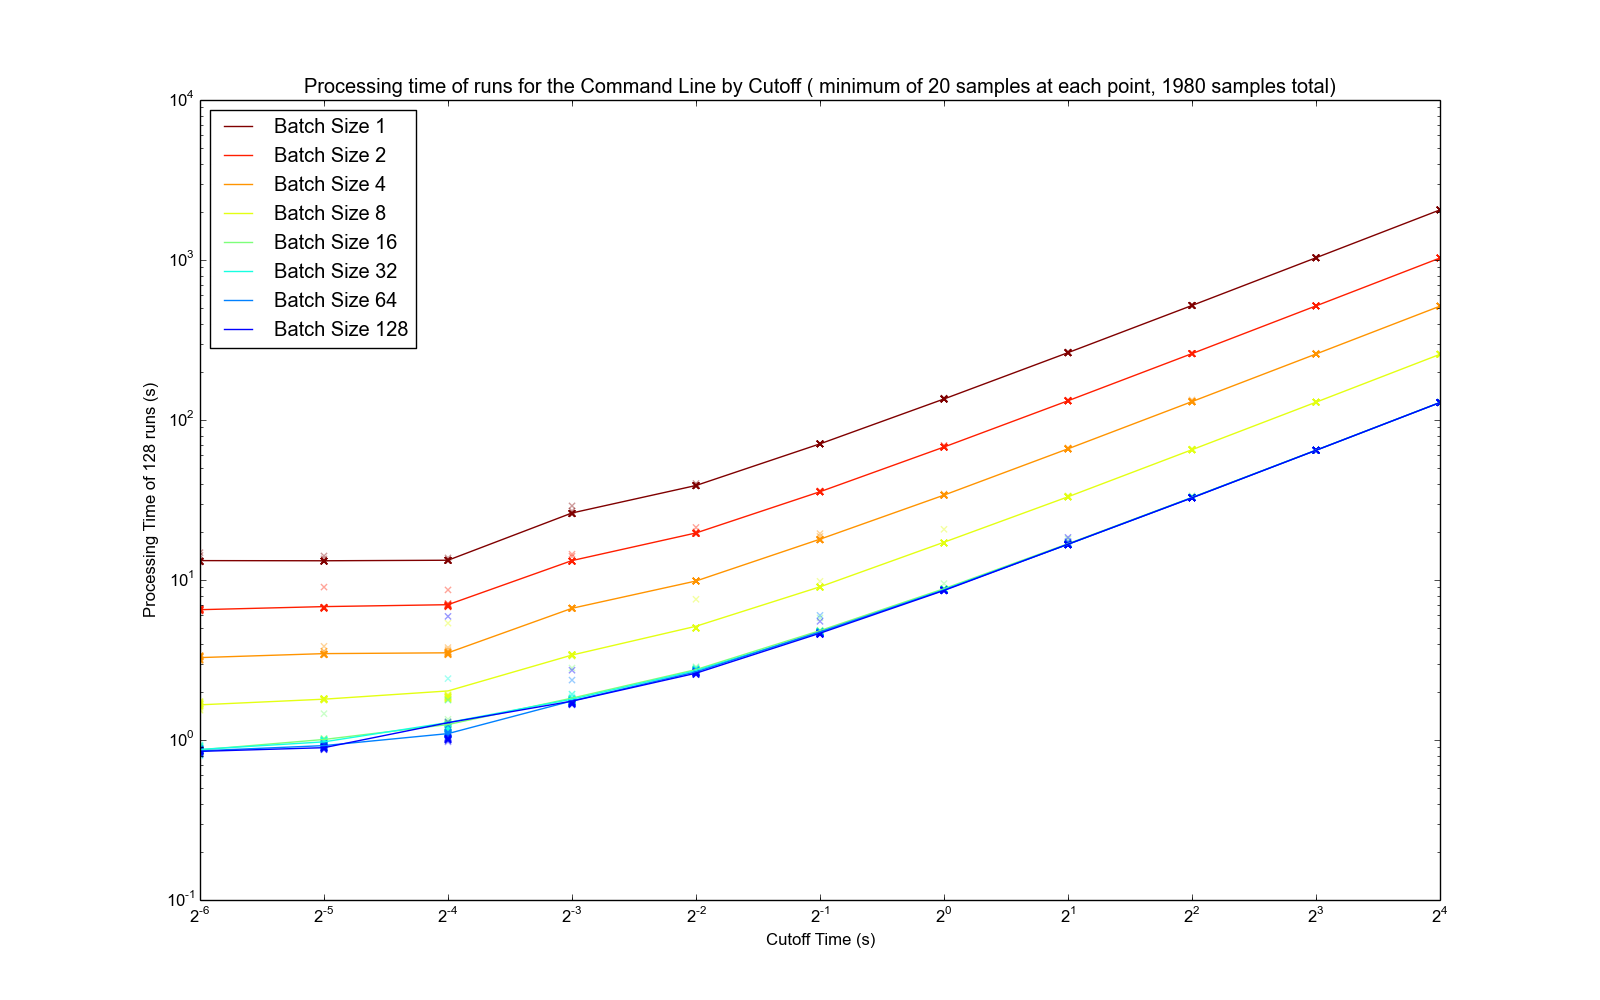
\includegraphics[width=480px]{img/plots/processTimeVersusCutoffTime-cli}
  %\caption{CLI TAE}

\end{subfigure}%
\begin{subfigure}
  \centering
  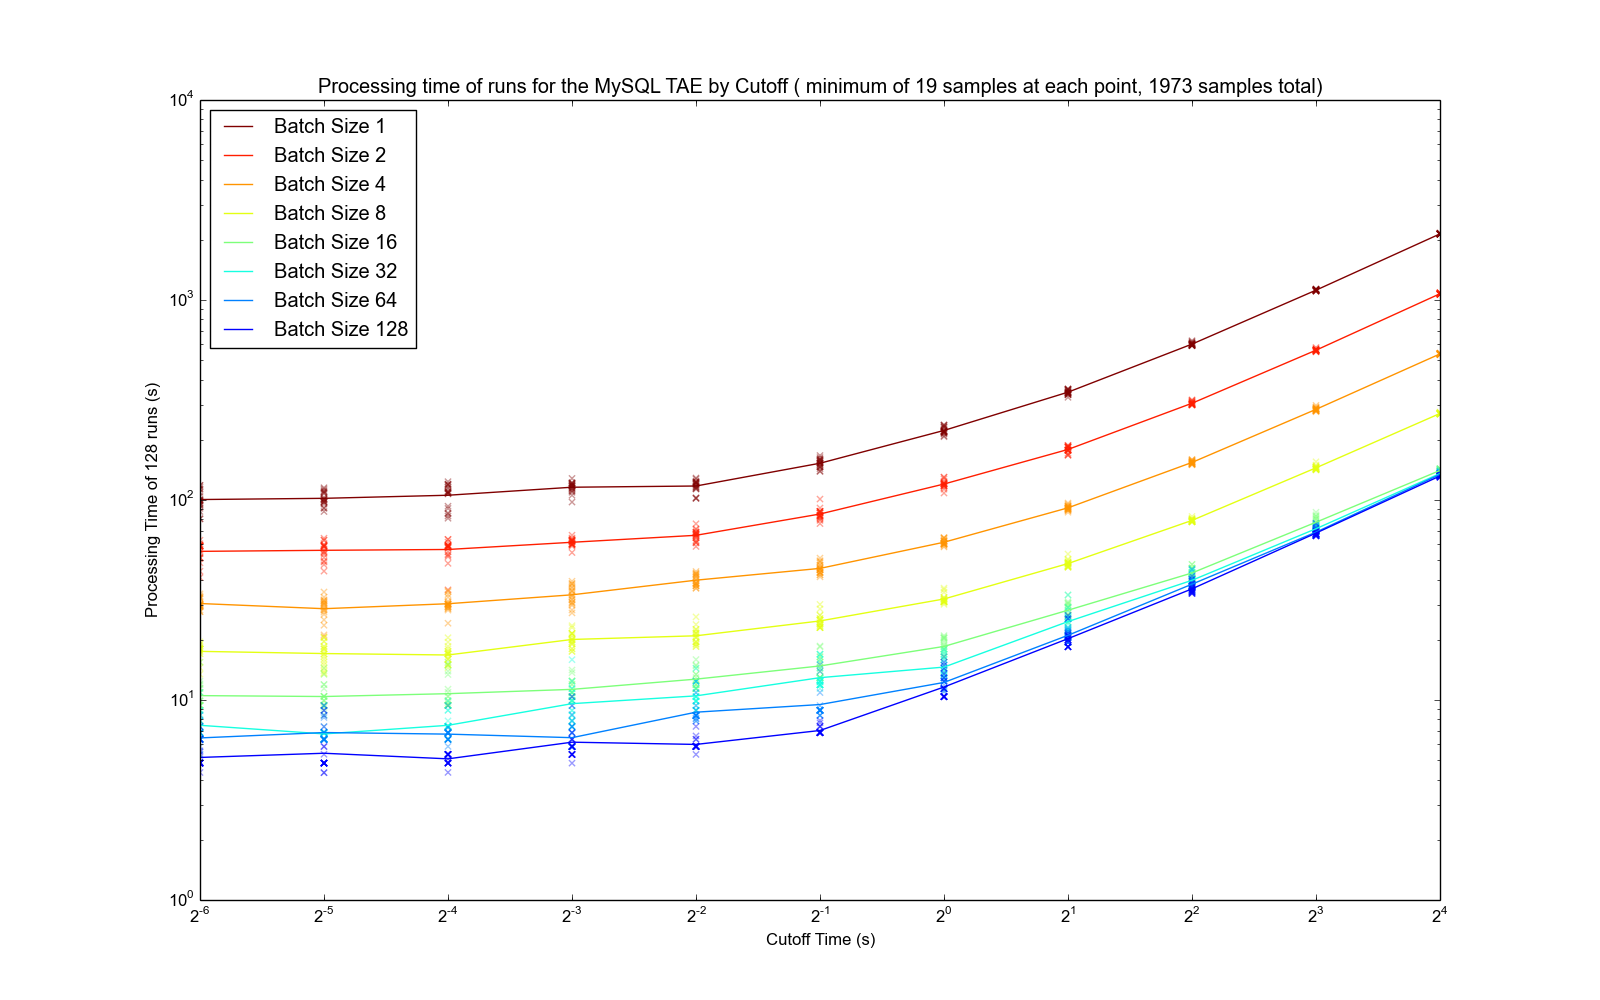
\includegraphics[width=480px]{img/plots/processTimeVersusCutoffTime-mysql}
  %\caption{MYSQLDB TAE}
  
\end{subfigure}
\caption{Processing Time of different batch sizes as a function of cutoff CLI (top/left) versus MySQL (bottom/right)}
\label{processTimeVersusCutoffTime}
\end{figure}


Figure \ref{processTimeVersusCutoffTime} on page \pageref{processTimeVersusCutoffTime} suggests the following:

\begin{enumerate}

\item The command line runs have much lower variance that the MySQL runs, probably due to the fact that there is less reliance on polling.

\item Increasing the batch size past 16 doesn't make much difference for the command line Target Algorithm Evaluator, but for the MySQL Target Algorithm Evaluator it makes a difference. This is probably due to the reduction in number of trips required to the database and the way that polling is implemented.

\item For the command line, runs less than about $2^{-4}$ seconds are dominated by overheads, where as for MySQL it is less clear but the graph tends to flatten around $2^{-2}$.

\end{enumerate}


\begin{figure}
\centering
\begin{subfigure}
  \centering
  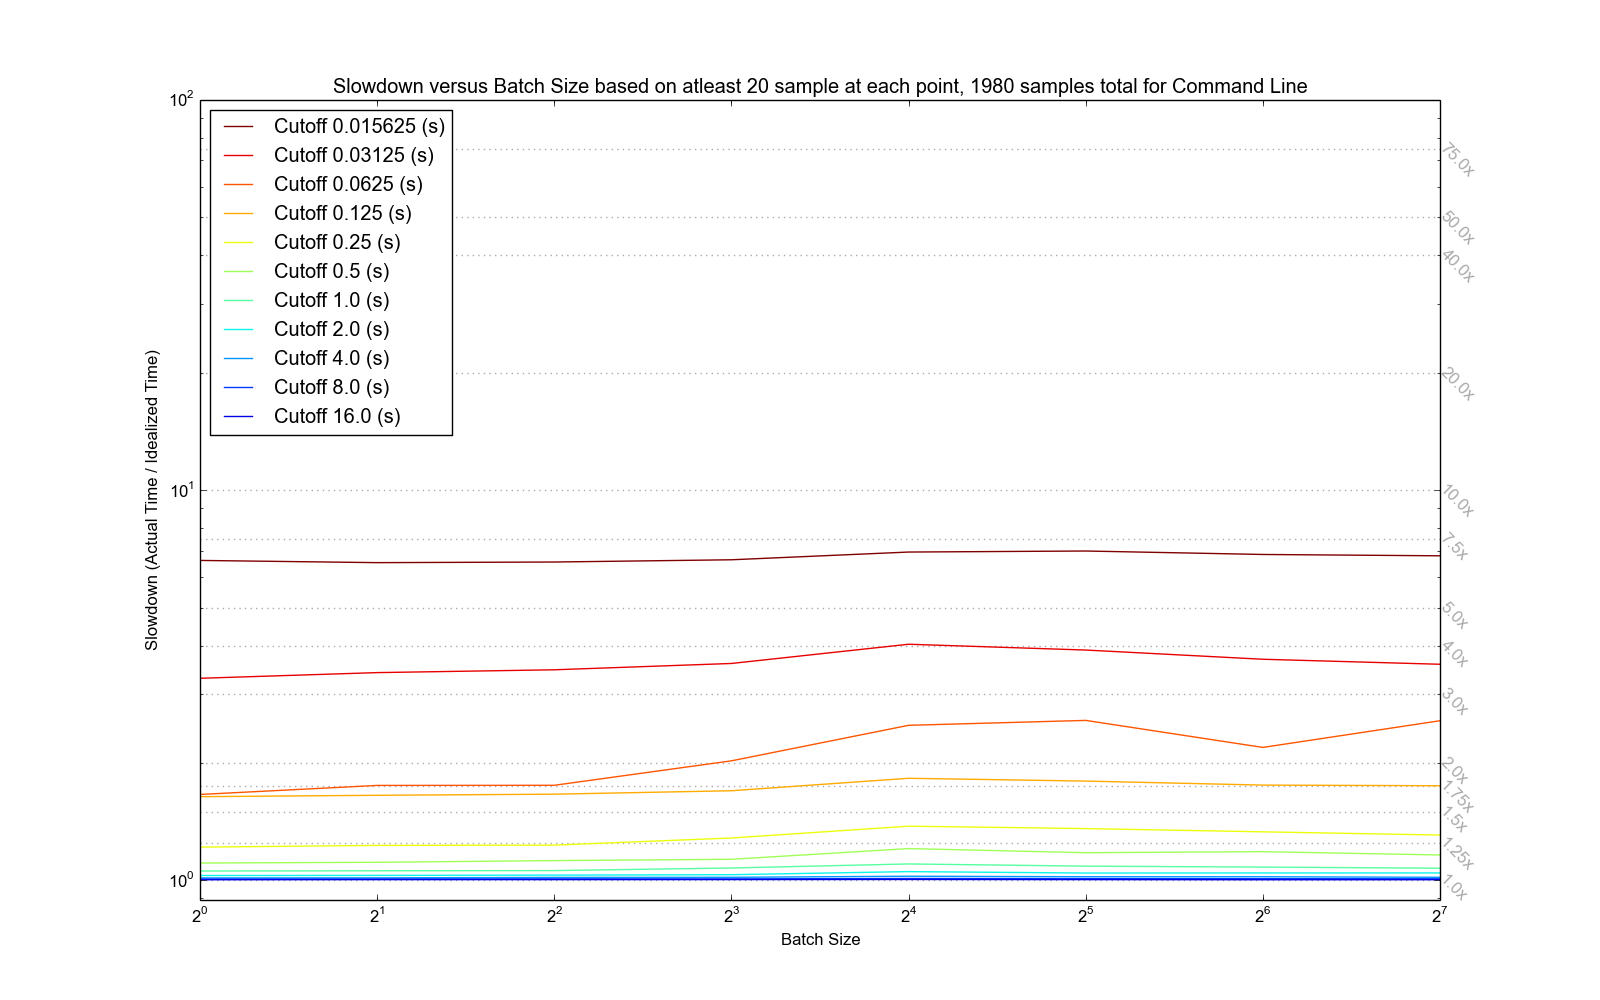
\includegraphics[width=480px]{img/plots/overheadVsBatchSize-cli}
  %\caption{CLI TAE}

\end{subfigure}%
\begin{subfigure}
  \centering
  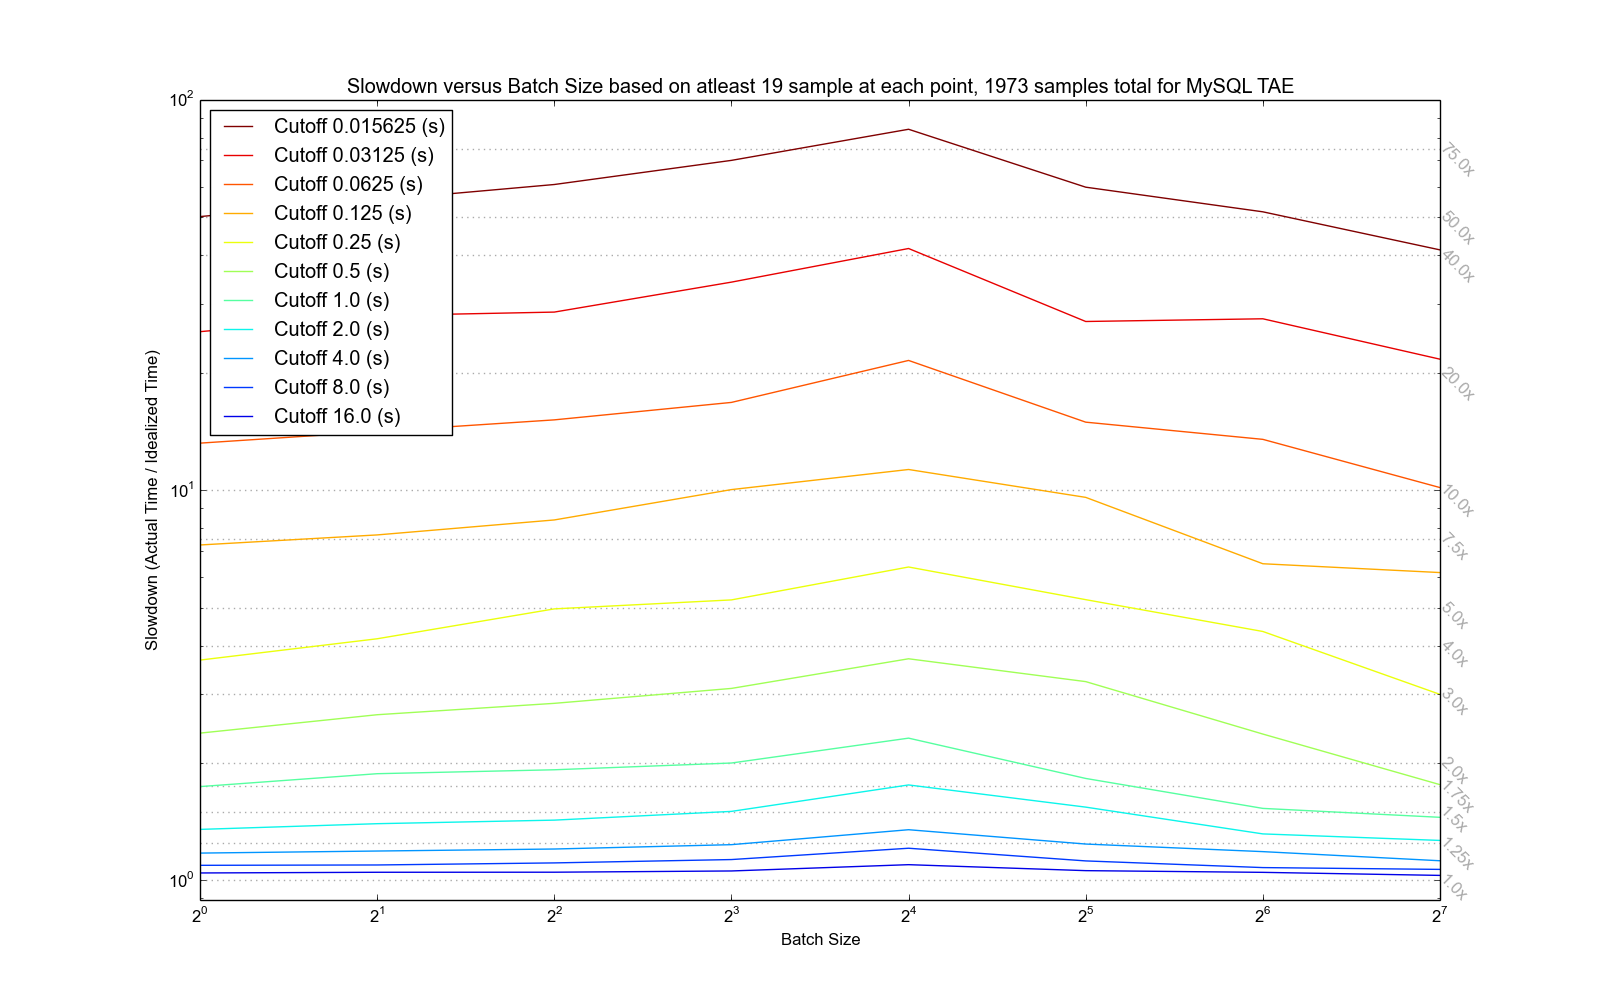
\includegraphics[width=480px]{img/plots/overheadVsBatchSize-mysql}
  %\caption{MYSQLDB TAE}

\end{subfigure}
\caption{Slowdown of different cutoff times as a function of batch size CLI (top/left) versus MySQL (bottom/right)}
\label{overheadBatch}
\end{figure}


In Figure \ref{overheadBatch} we can see how much slowdown the competing TAEs experience, in this case we have grouped the runs by cutoff, instead of batch size and suggests the following:

\begin{enumerate}

\item The slowdown experienced by runs seems mostly affected by the cutoff time, in the Command Line Target Algorithm Evaluator, except for some increased variation in the 0.0625 (s) case, the lines are mostly distinctively flat. 

\item In the MySQL Target Algorithm Evaluator case, the slowdowns are a factor of 10 slower for smaller batches, and even for the longest runs of 16.0 (s) still noticeably above 1$\times$.

\item In the MySQL case, batch size does have noticeable impact on overhead, up until a batch size of 16, the process becomes less efficient, and afterwards becomes more efficient. In general the batches of 128 have less slowdown than batches of 1. The improved efficiency after a batch size of 16 makes sense due to less polling of the database and potentially more efficient worker utilization, the decline prior to 16 is unclear at this time. 

\end{enumerate}




\section{Known Issues \& Future}

\label{sec:known-issues}
\begin{description}

\item[Instance Specific Information not hashed] Instance specific information won't form part of the hash. This is because the key to an instance is an instance name, but it's unclear whether this should be true in a database or not. 

\item[Instance features not supported] Instance features are not supported (instance features that exist in the AEATK application, will not be available on the worker). This could be fixed if needed.

%\item[Rename Columns] to better map to AEATK names. Right now they are inconsistent and it's unclear how they map and in some cases this is inconsistent. 

\item[Better Killed Run Support] could include the following mechanism. Add a new column, max\_observered\_runtime. This column simply shows the maximum observer runtime thus far. When we are observing runs, we always observe this column for the runtime, and when we update the database we always take the MAX of the current value and our value. When retrieving runs from the database, if we see that the run is \textbf{KILLED}, if we didn't request that it is killed, we will resubmit it as \texttt{NEW}. However, we will still report the previously seen value, and if it is killed by us we will then kill it in the database.

\item[Workers may hang if there is a high load on AEATK application] This occurs if the AEATK application has high CPU utilization and attempts to reclaim jobs from dead workers. This may hang other workers who attempt to do a similar check.

%\item[Migration Utility] this is necessary because the hashes need to be recomputed every time. One possibility is to read the runs into Java and then update the DB again with the correct hashes. This is actually somewhat of a burden to write and time consuming. A perhaps better approach is to create a stored procedure in the database to do the hashing for us. 

\end{description}



\section{Thoughts for Developers}

This section outlines random thoughts, musings, ideas that people who have to investigate the internals of the MySQL Target Algorithm Evaluator might find useful. It should go without saying that you should be very familiar with the AEATK API before attempting to digest this, and you should be very familiar with MySQL, and at least somewhat familiar with Java Concurrent Programming, lest this whole section appear to be incoherent ramblings.

\begin{itemize}

\item The use of \texttt{GET\_LOCK()} prior to retrieving the runs on a worker is unfortunately due to a mysterious performance issue that I could not solve. Essentially randomly sporadic freeze occurs that causes database performance to tank. For more details see: \url{http://forums.mysql.com/read.php?24,607838,607838\#msg-607838}. 

\item I would personally recommend avoiding adding more complicated logic to the retrieval of runs from the database by the worker. For instance more priority levels, or a more complicated ordering mechanisms would make the queries much more expensive. Presently it is believed that the SELECT query can be answered by only an index lookup only. One rule in MySQL, is that you can only have one column in an \texttt{ORDER BY} clause for an index to work efficiently, and we use it for FIFO ordering of runs.

\item I have no idea why I didn't put most things in the \texttt{RunToken} instead of in the Map for \texttt{MySQLPersistenceClient}, it does make zero sense.

\item A large literature exists suggesting that queues in MySQL are a bad idea. In some ways they are correct but note that most of the objections have been mitigated. Firstly we don't use \texttt{SELECT... FOR UPDATE}. Secondly the updates are atomic and done in a single batch \footnote{Which is odd because in MySQL you can't SELECT and UPDATE a table at the same time, but for some reason this query works, I suspect it's because an internal temporary table is made}. Fourthly there are advantages to using MySQL, and because the data being collected generally only has a short life span most of the standard objections do not apply (for instance it isn't the case that the tables grow without bound over months or years).

\item It is strongly recommended that you read \emph{High Performance MySQL 3rd Edition} if you are going to tinker with performance.

\item Most of the defaults and the settings are old and very, very conservative. They were chosen by simply observing good performance, noticing that the database locked up, and then doubling their values. The \texttt{GET\_LOCK()} strategy seems to have been a silver bullet for this, and so it's possible the settings could be made far more aggressive.

\item The indexes on the \textbf{runs} table seem to be counter intuitive, their purpose is primarily to act as covering indexes for queries \url(http://en.wikipedia.org/wiki/Database\_index\#Covering\_index), so even though they aren't very effective and segmenting the data, they can make things very fast. In fact while writing this manual a performance bug was detected related to this. During a migration of a very large database, the estimated time to complete the migration (repair hashes), decreased linearly for several hours implying that the runs were being processed at a constant rate. Eventually when 55\% of the runs were corrected, MySQL decided to switch indexes, this caused the queries to become a thousand times more expensive. We fixed this using an \texttt{USE INDEX} query but note the difference:

\begin{verbatim}

mysql> SELECT runID,1 AS priority
		 FROM dsmac_cli_runs_runs USE INDEX (status2)
		 WHERE status="PAUSED"
		  AND priority="NORMAL"
	   ORDER BY runID
	   LIMIT 1;
		  
+----------+----------+
| runID    | priority |
+----------+----------+
| 12825485 |        1 |
+----------+----------+
1 row in set (0.00 sec)

mysql> SELECT runID,1 AS priority
		 FROM dsmac_cli_runs_runs
		 WHERE status="PAUSED"
		  AND priority="NORMAL"
	   ORDER BY runID
	   LIMIT 1;
		  
+----------+----------+
| runID    | priority |
+----------+----------+
| 12825735 |        1 |
+----------+----------+
1 row in set (5.77 sec)

\end{verbatim}





\end{itemize}

%%%%%%%%%%%%%%%%%%%%%%%%%%%%%%%%%%%%%%%%%%%%%%%%%%%%%%%%%%%%%%%%%%%%
\section{Acknowledgements}
%%%%%%%%%%%%%%%%%%%%%%%%%%%%%%%%%%%%%%%%%%%%%%%%%%%%%%%%%%%%%%%%%%%%

Special thanks to Daniel Geschwender who implemented a number of features that made them much better to use. Also to Chris Thronton, Alex Fr\'echette, Richy Chen, Alim Virani, Chris Cameron, and Frank Hutter for feedback. Finally to people within \#mysql on Freenode, who were very helpful in sorting out the performance problems.


\section{Appendix I - Sample MySQL Configuration} 
\label{appendix:sampleconf}

\begin{bclogo}[logo=\bcattention, couleurBarre=red, noborder=true]{Important!}

The following is our current MySQL Configuration for MySQL 5.5. It \emph{disables} binary logging and as such if the database loses power there would be no backup or redundancy available. This is appropriate for our use cases, but may not be appropriate for yours.

\end{bclogo}


\begin{verbatim}
#This my.cnf file was created by Steve Ramage <seramage@cs.ubc.ca>
#It is based on the configuration of our local arrowdb database server
#and a read through of High Performance MySQL 3rd Edition, Chapter 8.



#Important Note: Binary logging is disabled, it is largely expected that 
#few if any users would benefit from any kind of replication and/or
#point-in-time recovery. as such we disabled it


[client]
port            = 3306
socket          = /var/run/mysqld/mysqld.sock

# Here is entries for some specific programs
# The following values assume you have at least 32M ram

# This was formally known as [safe_mysqld]. Both versions are currently parsed.
[mysqld_safe]
socket          = /var/run/mysqld/mysqld.sock
nice            = 0

[mysqld]
#
# * Basic Settings
#
user            = mysql
pid-file        = /var/run/mysqld/mysqld.pid
socket          = /var/run/mysqld/mysqld.sock
port            = 3306
basedir         = /usr
#datadir                = /var/lib/mysql
datadir         = /data/db/mysql
tmpdir          = /tmp

lc-messages-dir = /data/db/mysql


skip-external-locking

#
# Instead of skip-networking the default is now to listen only on
# localhost which is more compatible and is not less secure.
#bind-address           = 127.0.0.1
bind-address            = 0.0.0.0

# This replaces the startup script and checks MyISAM tables if needed
# the first time they are touched
myisam-recover         = BACKUP

server-id=1
slow-query-log=1
default-storage-engine=InnoDB

#We can expect MANY clients to connect at times with many threads

max_connections=22000
max_connect_errors=10000
thread_cache_size=256


#InnoDB Options
innodb = FORCE

#Set this to 80% of RAM
innodb_buffer_pool_size = 16G 

innodb_log_file_size = 1G
innodb_log_buffer_size = 8M

innodb_file_per_table = 1
innodb_flush_method = O_DIRECT
innodb_flush_log_at_trx_commit=2

innodb_file_format=Barracuda
innodb-file-per-table = true

#Couldn't set innodb_io_capacity as I wasn't able to login to disk directly
#Suspect RAID6 may perform poorly, unsure though

#Other settings taken from arrow (not tuned)
tmp_table_size=128M

sort_buffer_size=16M
join_buffer_size=256M
query_cache_size=128M
query_cache_limit=2M
max_allowed_packet=64M
table_cache=2048


#Key Buffer Size  (MyISAM options)
myisam_sort_buffer_size=256M
read_rnd_buffer_size=4M
read_buffer_size=2M
key_buffer = 256M
key_buffer_size=64M

#Query Cache 

#Taken from High Performance MySQL (3rd Edition p 343)

tmp_table_size = 32M
max_heap_table_size = 32M


open_files_limit = 65535

[mysqldump]
quick
quote-names
max_allowed_packet      = 16M

[mysql]
no-auto-rehash # faster start of mysql but no tab completition

[isamchk]
key_buffer              = 16M

#
# * IMPORTANT: Additional settings that can override those from this file!
#   The files must end with '.cnf', otherwise they'll be ignored.
#
#!includedir /etc/mysql/conf.d/

\end{verbatim}


%Also special thanks to Alexandre Fr\'echette




\renewcommand{\bibsection}{\section{References}}
\bibliographystyle{apalike}
\bibliography{short,frankbib}


\end{document}

